%% 使用 njuthesis 文档类生成南京大学学位论文的示例文档
%%
%% 作者:胡海星,starfish (at) gmail (dot) com
%% 项目主页: http://haixing-hu.github.io/nju-thesis/
%%
%% 本样例文档中用到了吕琦同学的博士论文的提高和部分内容,在此对他表示感谢。
%%
\documentclass[master]{njuthesis}
%% njuthesis 文档类的可选参数有:
%%   nobackinfo 取消封二页导师签名信息。注意,按照南大的规定,是需要签名页的。
%%   phd/master/bachelor 选择博士/硕士/学士论文

% 使用 blindtext 宏包自动生成章节文字
% 这仅仅是用于生成样例文档,正式论文中一般用不到该宏包
\usepackage[math]{blindtext}

%%%%%%%%%%%%%%%%%%%%%%%%%%%%%%%%%%%%%%%%%%%%%%%%%%%%%%%%%%%%%%%%%%%%%%%%%%%%%%%
% 设置《国家图书馆封面》的内容,仅博士论文才需要填写

% 设置论文按照《中国图书资料分类法》的分类编号
\classification{}
% 论文的密级。需按照GB/T 7156-2003标准进行设置。预定义的值包括:
% - \openlevel,表示公开级:此级别的文献可在国内外发行和交换。
% - \controllevel,表示限制级:此级别的文献内容不涉及国家秘密,但在一定时间内
%   限制其交流和使用范围。
% - \confidentiallevel,表示秘密级:此级别的文献内容涉及一般国家秘密。
% - \clasifiedlevel,表示机密级:此级别的文献内容涉及重要的国家秘密 。
% - \mostconfidentiallevel,表示绝密级:此级别的文献内容涉及最重要的国家秘密。
% 此属性可选,默认为\openlevel,即公开级。
\securitylevel{\controllevel}
% 设置论文按照《国际十进分类法UDC》的分类编号
% 该编号可在下述网址查询:http://www.udcc.org/udcsummary/php/index.php?lang=chi
\udc{}
% 国家图书馆封面上的论文标题第一行,不可换行。此属性可选,默认值为通过\title设置的标题。
\nlctitlea{}
% 国家图书馆封面上的论文标题第二行,不可换行。此属性可选,默认值为空白。
\nlctitleb{}
% 国家图书馆封面上的论文标题第三行,不可换行。此属性可选,默认值为空白。
\nlctitlec{}
% 导师的单位名称及地址
\supervisorinfo{南京大学计算机科学与技术系~~南京市汉口路22号~~210093}
% 答辩委员会主席
\chairman{~~教授}
% 第一位评阅人
\reviewera{~~教授}
% 第二位评阅人
\reviewerb{~~副教授}
% 第三位评阅人
\reviewerc{~~教授}
% 第四位评阅人
\reviewerd{~~研究员}

%%%%%%%%%%%%%%%%%%%%%%%%%%%%%%%%%%%%%%%%%%%%%%%%%%%%%%%%%%%%%%%%%%%%%%%%%%%%%%%
% 设置论文的中文封面

% 论文标题,不可换行
\title{基于神经网络的文本向量表示和建模研究 }
% 论文作者姓名
\author{牛力强}
% 论文作者联系电话
\telphone{15996276729}
% 论文作者电子邮件地址
\email{simpleniulq2013@gmail.com}
% 论文作者学生证号
\studentnum{MF1333036}
% 论文作者入学年份(年级)
\grade{2013}
% 导师姓名职称
\supervisor{戴新宇~~副教授}
% 导师的联系电话
\supervisortelphone{+86 18913825156}
% 论文作者的学科与专业方向
\major{计算机技术}
% 论文作者的研究方向
\researchfield{自然语言处理}
% 论文作者所在院系的中文名称
\department{计算机科学与技术系}
% 论文作者所在学校或机构的名称。此属性可选,默认值为``南京大学''。
\institute{南京大学}
% 论文的提交日期,需设置年、月、日。
\submitdate{2016年5月10日}
% 论文的答辩日期,需设置年、月、日。
\defenddate{2016年6月1日}
% 论文的定稿日期,需设置年、月、日。此属性可选,默认值为最后一次编译时的日期,精确到日。
%% \date{2013年5月1日}

%%%%%%%%%%%%%%%%%%%%%%%%%%%%%%%%%%%%%%%%%%%%%%%%%%%%%%%%%%%%%%%%%%%%%%%%%%%%%%%
% 设置论文的英文封面

% 论文的英文标题,不可换行
\englishtitle{A Research on Text Vector Representations and Modelling based on Neural Networks}
% 论文作者姓名的拼音
\englishauthor{NIU Li-Qiang}
% 导师姓名职称的英文
\englishsupervisor{Associate Professor DAI Xin-Yu}
% 论文作者学科与专业的英文名
\englishmajor{Computer Technology}
% 论文作者所在院系的英文名称
\englishdepartment{Department of Computer Science and Technology}
% 论文作者所在学校或机构的英文名称。此属性可选,默认值为``Nanjing University''。
\englishinstitute{Nanjing University}
% 论文完成日期的英文形式,它将出现在英文封面下方。需设置年、月、日。日期格式使用美国的日期
% 格式,即``Month day, year'',其中``Month''为月份的英文名全称,首字母大写;``day''为
% 该月中日期的阿拉伯数字表示;``year''为年份的四位阿拉伯数字表示。此属性可选,默认值为最后
% 一次编译时的日期。
\englishdate{Mar 1, 2016}

%%%%%%%%%%%%%%%%%%%%%%%%%%%%%%%%%%%%%%%%%%%%%%%%%%%%%%%%%%%%%%%%%%%%%%%%%%%%%%%
% 设置论文的中文摘要

% 设置中文摘要页面的论文标题及副标题的第一行。
% 此属性可选,其默认值为使用|\title|命令所设置的论文标题
% \abstracttitlea{数据中心网络模型研究}
% 设置中文摘要页面的论文标题及副标题的第二行。
% 此属性可选,其默认值为空白
% \abstracttitleb{}

%%%%%%%%%%%%%%%%%%%%%%%%%%%%%%%%%%%%%%%%%%%%%%%%%%%%%%%%%%%%%%%%%%%%%%%%%%%%%%%
% 设置论文的英文摘要

% 设置英文摘要页面的论文标题及副标题的第一行。
% 此属性可选,其默认值为使用|\englishtitle|命令所设置的论文标题
\englishabstracttitlea{A Research on Text Vector Representations and Modelling}
% 设置英文摘要页面的论文标题及副标题的第二行。
% 此属性可选,其默认值为空白
\englishabstracttitleb{based on Neural Networks}

%%%%%%%%%%%%%%%%%%%%%%%%%%%%%%%%%%%%%%%%%%%%%%%%%%%%%%%%%%%%%%%%%%%%%%%%%%%%%%%
\begin{document}

%%%%%%%%%%%%%%%%%%%%%%%%%%%%%%%%%%%%%%%%%%%%%%%%%%%%%%%%%%%%%%%%%%%%%%%%%%%%%%%

% 制作国家图书馆封面(博士学位论文才需要)
%\makenlctitle
% 制作中文封面
\maketitle
% 制作英文封面
\makeenglishtitle


%%%%%%%%%%%%%%%%%%%%%%%%%%%%%%%%%%%%%%%%%%%%%%%%%%%%%%%%%%%%%%%%%%%%%%%%%%%%%%%
% 开始前言部分
\frontmatter

%%%%%%%%%%%%%%%%%%%%%%%%%%%%%%%%%%%%%%%%%%%%%%%%%%%%%%%%%%%%%%%%%%%%%%%%%%%%%%%
% 论文的中文摘要
\begin{abstract}

文本表示与建模是自然语言处理领域中的基础任务。传统的文本表示方法主要是基于词袋模型,将文本映射至一个由所有存在的词项组成的一个高维0/1空间,若出现,则对应维度置为1,否则置为0。词袋模型的好处在于简单高效,容易扩展,但同时也面临众多严重的问题,如维度灾难、数据稀疏表示、缺失语义表达能力等。近年来随着大数据和深度学习技术在语音、图像、生物信息等领域取得重大的成果,研究者们也开始将深度神经网络技术应用到自然语言处理领域。特别地,随着2008年Collobert和Weston将基于深度神经网络的词向量表示应用到各类自然语言处理任务以及2013年谷歌研究员基于神经网络语言模型来学习分布式词向量表示,越来越多基于神经网络模型来学习文本向量表示的方法出现。

本文集中对基于神经网络语言模型的文本向量表示和主题建模问题进行了研究。首先简单介绍了传统N-Gram统计语言模型和基于神经网络的语言模型,并且回顾传统词向量表示方法以基于神经网络语言模型学习分布式词向量表示模型Word2Vec。随后基于这些基础模型与方法,本文对其进行了多方面的扩展:

\begin{enumerate}
\item 提出主题语义向量学习模型Topic2Vec:借助于潜在狄利克雷分布(Latent Dirichlet Allocation, LDA)挖掘词的主题信息,扩展Word2Vec模型来学习主题的语义向量表示。相比原始LDA中词、主题和文档均以空间下标(Indices)来表示而且词与主题之间的关系采用条件概率来衡量,Topic2Vec将词及其主题映射至同一个语义向量空间,词与主题之间关系可以直接采用余弦相似度来度量。
\item 提出能够联合学习词及其属性向量表示的统一学习框架:将词向量表示学习模型Word2Vec扩展到联合学习词及其属性语义向量表示的统一框架。相比单一模型的学习能力,联合学习框架使得词与其属性在学习过程中相互促进可以得到更好的语义向量表示。
\item 融合词向量与主题模型:结合词向量表示可以表征词的句法和语义信息的特性和LDA主题模型在收敛速度、收敛结果以及主题一致性方面的问题,将词向量表示应用到LDA中来提升原有主题模型的效果。特别地,提出了词向量聚类先验LDA、上下文感知LDA和词向量加强LDA。
\end{enumerate}
针对扩展之后的模型方法,本文分别给出了原理和实现,并且进行了多方面的实验评估,结果表明扩展之后的模型方法表现更好。


% 中文关键词。关键词之间用中文全角分号隔开,末尾无标点符号。
\keywords{自然语言处理;文本表示;深度学习;神经网络;文本建模;主题模型;词向量;主题;文档;框架;潜在狄利克雷分布}
\end{abstract}

%%%%%%%%%%%%%%%%%%%%%%%%%%%%%%%%%%%%%%%%%%%%%%%%%%%%%%%%%%%%%%%%%%%%%%%%%%%%%%%
% 论文的英文摘要
\begin{englishabstract}

Text representations and modelling are fundamental tasks in Natural Langauge Processing (NLP) area. Traditionally, these methods of text representations are based on Bag-of-Words (BOW) models, which could map arbitrary text into a high-dimensional binary space constructed by existing terms. If one term occurs, then corresponding index will be set to 1, otherwise 0. Even BOW models are simple, efficient, and scalable, they suffer from disadvantages such as the curse of dimensionality, data sparsity, and inability to capture semantic information. Recently, with the significant development of appling big data and deep learning technologies in speech, image, and bioinformatics areas, researcher start taking the usage of deep neural networks (DNN) to NLP area. In particular, Collobert and Westion applied DNN-based word vector representations in all kinds of NLP tasks in 2008, Google researcher learned distributed word vector representations with neural network language models (NNLMs) in 2013, and now there is an increasing number of  text embedding methods based on neural networks.

This paper focuses on studying NNLM-based text vector representations and topic models. First we briefly introduce traditional N-Gram statistical language models and neural network language models, also review some traditional methods of word representations and NNLM-based Word2Vec model which can learn distributed word representations. Then this paper extends these basic models and methods in the following aspects:

\begin{enumerate}
\item Proposed topic representation learning model Topic2Vec: with the help of topic information mined by Latent Dirichlet Allocation (LDA), we extend Word2Vec to Topic2Vec for learning distributed topic representations. Compared to LDA, in which words, topics, and documents are represented as indices, and conditional probabilities measure the relationship between words and topics, Topic2Vec embeds words and topics into the same semantic space, meanwhile we can immediately use cosine similarity to measure the words and topics.
\item A proposed unified framework for jointly learning distributed representations of word and attributes: we extend Word2Vec to a unified framework for jointly learning distributed representations of word and attributes. Compare to capacity of single model, this unified framework has the benefit that word and attributes help each other during the learning process. 
\item Fusing word embeddings and topic models: by intergrating the characteristic of syntactic and semantic information in word embeddings and the challenges of convergence rate, results and topic coherence in LDA, we apply word embeddings into the LDA for improving topic models. In particular, we propose word embedding cluster prior LDA, context-aware LDA, and word embedding enhanced LDA.
\end{enumerate}
To these extended models and methods, this paper provides basic principles and realizations respectively, and also conduct various experiments and evaluation. Finally, experiment results show that our extended models and methods perform better.


% 英文关键词。关键词之间用英文半角逗号隔开,末尾无符号。
\englishkeywords{Natural Language Processing (NLP), Text Representation, Deep Learning, Neural Networks, Text Modelling, Topic Models, Word Embeddings, Topic, Document, Framework, Latent Dirichlet Allocation (LDA)}
\end{englishabstract}

%%%%%%%%%%%%%%%%%%%%%%%%%%%%%%%%%%%%%%%%%%%%%%%%%%%%%%%%%%%%%%%%%%%%%%%%%%%%%%%
% 论文的前言,应放在目录之前,中英文摘要之后
%
\begin{preface}

在机器学习系统的设计过程中,数据的表示是一项基础工程,好的数据表示方法能够提升整个系统的性能。传统思路下研究者们重点关注如何设计出更好的模型系统来达到更好的结果,而数据的表示则大多采用人工设计的方法。但是,近年来随着互联网大数据时代的到来以及2006年深度学习技术的兴起,大数据及数据表示方法在机器学习系统中扮演的角色越来越重要。特别地,基于深度学习技术,采用多层神经网络学习数据的层次化表示迅速成为一大研究热点,而且已经取得不俗的成果。

在自然语言处理领域中,文本表示是一项基础任务,好的文本表示方法将直接有益于后续各项自然语言处理任务。传统的文本表示方法主要是基于词袋模型,即将所有的词项组成高维0/1特征空间,若词项出现,则对应维度置为1,否则置为0。词袋模型的好处在于简单高效,但是面临众多严重的问题,如维度灾难、数据稀疏、缺失语义表达能力等。而最新的基于深度学习的文本表示方法通过多层神经网络的学习将文本中的多层结构(词、短语、句子、段落、文档等)映射至一个低维连续的空间,任意的文本都对应一个低维连续值的向量。因此,新的深度学习文本表示方法完美的克服了原来词袋模型的弊端,而且在各类自然语言处理任务中取得了最好的结果。如基于神经网络的机器翻译、基于神经网络的文本分类、情感分析、复述识别等等\cite{mikolov2013efficient,collobert2008unified,socher2011dynamic}。

本文集中对基于神经网络语言模型的文本向量表示和主题建模问题进行了研究。首先简单介绍了传统N-Gram统计语言模型和基于神经网络的语言模型,并且回顾传统词向量表示方法以基于神经网络语言模型学习分布式词向量表示模型Word2Vec。随后基于这些基础模型与方法,本文对其进行了多方面的扩展:

\begin{enumerate}
\item 提出主题语义向量学习模型Topic2Vec:借助于潜在狄利克雷分布(Latent Dirichlet Allocation, LDA)挖掘词的主题信息,扩展Word2Vec模型来学习主题的语义向量表示。相比原始LDA中词、主题和文档均以空间下标(Indices)来表示而且词与主题之间的关系采用条件概率来衡量,Topic2Vec将词及其主题映射至同一个语义向量空间,词与主题之间关系可以直接采用余弦相似度来度量。
\item 提出能够联合学习词及其属性向量表示的统一学习框架:将词向量表示学习模型Word2Vec扩展到联合学习词及其属性语义向量表示的统一框架。相比单一模型的学习能力,联合学习框架使得词与其属性在学习过程中相互促进可以得到更好的语义向量表示。
\item 融合词向量与主题模型:结合词向量表示可以表征词的句法和语义信息的特性和LDA主题模型在收敛速度、收敛结果以及主题一致性方面的问题,将词向量表示应用到LDA中来提升原有主题模型的效果。特别地,提出了词向量聚类先验LDA、上下文感知LDA和词向量加强LDA。
\end{enumerate}
针对扩展之后的模型方法,本文分别给出了原理和实现,并且进行了多方面的实验评估,结果表明扩展之后的模型方法均表现更好。

\vspace{1cm}
\begin{flushright}
牛力强\\
2016年夏于南京大学
\end{flushright}

\end{preface}

%%%%%%%%%%%%%%%%%%%%%%%%%%%%%%%%%%%%%%%%%%%%%%%%%%%%%%%%%%%%%%%%%%%%%%%%%%%%%%%
% 生成论文目次
\tableofcontents

%%%%%%%%%%%%%%%%%%%%%%%%%%%%%%%%%%%%%%%%%%%%%%%%%%%%%%%%%%%%%%%%%%%%%%%%%%%%%%%
% 生成插图清单。如无需插图清单则可注释掉下述语句。
\listoffigures

%%%%%%%%%%%%%%%%%%%%%%%%%%%%%%%%%%%%%%%%%%%%%%%%%%%%%%%%%%%%%%%%%%%%%%%%%%%%%%%
% 生成附表清单。如无需附表清单则可注释掉下述语句。
\listoftables

%%%%%%%%%%%%%%%%%%%%%%%%%%%%%%%%%%%%%%%%%%%%%%%%%%%%%%%%%%%%%%%%%%%%%%%%%%%%%%%
% 开始正文部分
\mainmatter

%%%%%%%%%%%%%%%%%%%%%%%%%%%%%%%%%%%%%%%%%%%%%%%%%%%%%%%%%%%%%%%%%%%%%%%%%%%%%%%
% 学位论文的正文应以《绪论》作为第一章

\chapter{绪论}\label{chapter1_introduction}
\section{研究背景}\label{sec_chap1_background}

自然语言同语音、图像并列为人工智能研究领域的三大重要元素。特别地,自2006年Hinton提出深度学习技术\cite{hinton2006reducing}并且在机器学习以及人工智能领域取得重大突破。其中,语音识别、计算机视觉、图像处理等典型人工智能任务取得了重大进展与广泛应用。但是,不同于语音、图像等原始信号或者信息,自然语言是人类高度抽象之后的产物。因此,深度学习等机器学习技术在面对自然语言处理任务时依旧面临较大的挑战。

传统的自然语言处理任务包括了语言建模、机器翻译、文本分类、情感分析、句法分析、词性标注、命名实体识别、中文分词、复述识别、自动问答等等\cite{collobert2008unified}。传统的自然语言处理方法大多是将有监督(supervised)机器学习模型方法根据对应的任务加以修改应用。例如,基于短语的统计机器翻译采用双语平行语料,依据源语言与目标语言词对齐方法来构建翻译模型,之后基于翻译模型来将源语言翻译为目标语言\cite{chiang2005hierarchical};文本分类、情感分析、复述识别等都是将具体的任务转换为有监督机器学习中二分类或者多分类任务,不同的任务采取不同的特征提取方法,进而构建对应的分类器\cite{collobert2008unified};句法分析、中文分词等序列标注任务部分采用条件随机场等图模型方法,基于特征模板来提取特征进而构造有监督分类器来进行参数学习\cite{lafferty2001conditional,zhao2006improved}。可以看到传统自然语言处理处理的最大局限在于采用有监督的机器学习方法,而现实中有监督方法所需的标记语料是相对有限且人工成本昂贵。因此,传统有监督机器学习方法在自然语言处理任务中的效果并不理想依旧面临很大的问题与挑战。

在此背景下,诸多研究者意识到深度学习的下一个突破口是自然语言处理领域。深度学习在语音以及图像等领域的成果得益于多层神经网络基于大量的未标注语料中的层次特征表示学习能力。如在图像中,神经网络通过层次化的学习可以学习到像素(pixel)、边际(edge)、部分(part)、图像(image)的表示,之后通过这些不同层级的特征来构造分类器\cite{lee2009convolutional}。可以看到多层神经网络在处理图像时模拟人脑的处理过程,因此深度学习得以取得重大突破,语音识别也类似\cite{lee2009unsupervised}。因此,研究者将自然语言处理的突破寄望于深度学习。近年来,研究者也开始探索文本的层次化表示学习,并希望通过基于深度学习的文本表示方法来提升传统的自然语言处理任务。特别地,随着2008年Collobert和Weston将基于深度神经网络的词向量表示应用到各类自然语言处理任务\cite{collobert2008unified}以及2013年谷歌研究员基于神经网络语言模型来学习分布式词向量表示\cite{mikolov2013efficient},越来越多基于神经网络模型来学习文本向量表示的方法出现。

\section{研究目的与意义}\label{sec_chap1_motivations}

对文本包括词(Word)、主题(Topic)、句子(Sentence)、文档(Document)等进行建模在自然语言处理(Natural Language Processing, NLP)和信息检索(Information Retrieval, IR)领域是一项关键任务,其目的在于找到一类简短扼要的描述来表达文本的语义,使其能够促进大规模系统的高效处理并且有益于常见的任务,例如文本分类、聚类、摘要、相似性或者相关性估计。

在过去的几十年间,各种各样的模型和解决方法被提出来,例如词袋模型(Bag-of-Words, BOW)\cite{zhang2010understanding}、TF-IDF\cite{salton1986introduction}、潜在语义分析(Latent Semantic Analysis, LSA)\cite{landauer1998introduction}、概率潜在语义分析(Probabilistic Latent Semantic Analysis, PLSA)\cite{hofmann1999probabilistic}、潜在狄利克雷分布(Latent Dirichlet Allocation, LDA)\cite{blei2003latent}等。词袋模型的好处在于简单高效,但是面临众多严重的问题,如维度灾难、数据稀疏、缺失语义表达能力等。

近年来,基于深度学习的文本表示方法通过多层神经网络的学习将文本中的多层结构(词、短语、句子、段落、文档等)映射至一个低维连续的空间,每一种类型的文本都对应一个低维连续值的向量,如词向量(Word Embedding)。理论上基于神经网络的文本表示方法完美的克服了传统词袋模型的问题,而且在各类自然语言处理任务中取得了最好的结果\cite{collobert2008unified}。如基于Bengio等人在2003年提出的神经网络语言模型\cite{bengio2003neural},Mikolov等人在2013年提出了Word2Vec模型来学习分布式(distributed)词向量表示\cite{mikolov2013efficient,mikolov2013distributed,mikolov2013linguistic};Le和Mikolov在2014年提出学习句子和文档分布式向量表示的方法\cite{le2014distributed};Stanford大学Socher等人利用递归自编码器和动态池化(Pooling)技术来做复述识别取得目前最好的结果\cite{socher2011dynamic};Tang等人在2014年利用开发了基于深度学习技术的系统用于Twitter情感分类\cite{tang2014coooolll};还有各类基于递归神经网络和编码-解码器的统计机器翻译模型\cite{bahdanau2014neural,cho2014learning}。

综上可以看出,基于神经网络的文本表示与建模在克服传统方法缺点的同时,在各类自然语言处理任务中均取得较好甚至是最好的结果。但是,深度学习技术在NLP领域的应用远不止于此。基于近年来深度学习用于自然语言处理任务所取得的成果,本文集中对基于神经网络语言模型的文本向量表示和主题建模问题进行了研究。首先简单介绍了传统N-Gram统计语言模型和基于神经网络的语言模型,并且回顾传统词向量表示方法以基于神经网络语言模型学习分布式词向量表示模型Word2Vec。随后基于这些基础模型与方法,本文对其进行了多方面的扩展:

\begin{enumerate}
\item 提出主题语义向量学习模型Topic2Vec:借助于潜在狄利克雷分布(Latent Dirichlet Allocation, LDA)挖掘词的主题信息,扩展Word2Vec模型来学习主题的语义向量表示。相比原始LDA中词、主题和文档均以空间下标(Indices)来表示而且词与主题之间的关系采用条件概率来衡量,Topic2Vec将词及其主题映射至同一个语义向量空间,词与主题之间关系可以直接采用余弦相似度来度量。
\item 提出能够联合学习词及其属性向量表示的统一学习框架:将词向量表示学习模型Word2Vec扩展到联合学习词及其属性语义向量表示的统一框架。相比单一模型的学习能力,联合学习框架使得词与其属性在学习过程中相互促进可以得到更好的语义向量表示。
\item 融合词向量与主题模型:结合词向量表示可以表征词的句法和语义信息的特性和LDA主题模型在收敛速度、收敛结果以及主题一致性方面的问题,将词向量表示应用到LDA中来提升原有主题模型的效果。特别地,提出了词向量聚类先验LDA、上下文感知LDA和词向量加强LDA。
\end{enumerate}
针对扩展之后的模型方法,本文分别给出了原理和实现,并且进行了多方面的实验评估,结果表明扩展之后的模型方法表现更好。因此,尽管深度学习技术已经在文本表示与建模甚至是整个NLP领域做出不俗的成绩,但当我们面对具体的实际问题时候,仍需思考当前问题的不同之处以及现有方法的不足,对现有模型做出修改或者创新才能做到更好的效果。

\section{论文结构}\label{sec_chap1_outline}

本文旨在对深度学习技术在自然语言处理领域中文本表示与建模这一问题的应用做进一步的探索,从(1)学习主题向量表示、(2)联合学习词及其属性分布式表示和(3)融合词向量表示与主题模型等方面来进行扩展,分析了现有方法的不足之处,提出了自己的模型方法,分别给出了原理和实现并且进行了实验对比。

本文一共分为六章,后续章节安排如下:

\begin{itemize}
\item 第\ref{chapter2_nnlm_word_representations}章:语言模型与词向量表示。本章主要介绍本文的背景工作,包括传统N-Gram统计语言模型、Bengio等人在2003年提出的神经网络语言模型\cite{bengio2003neural}以及Mikolov等人在2013年提出的基于神经网络语言模型学习分布式词向量表示的模型Word2Vec\cite{mikolov2013efficient,mikolov2013distributed,mikolov2013linguistic}。
\item 第\ref{chapter3_topic_representations}章:学习主题的向量表示。本章主要工作是借助于潜在狄利克雷分布(Latent Dirichlet Allocation, LDA)挖掘到词的主题(Topic)信息,将Word2Vec扩展至学习分布式主题向量表示,并且提出了模型Topic2Vec。
\item 第\ref{chapter4_word_attributes}章:联合学习词和属性的向量表示。本章主要工作是将Word2Vec扩展到一个能够联合学习词(Word)和属性(Attributes)分布式向量表示的统一框架,其中重点引入了三类词属性:词元(Lemma)、主题(Topic)、文档(Document),基于该框架实现:(1)学习主题Topic的分布式表示、(2)学习文档Document的分布式表示和(3)利用词元Lemma和主题Topic信息来提升词向量表示。该框架不仅可以学习到属性的分布式表示,而且可以利用属性知识来提高原来词向量表示。另外,该框架易于扩展,可以学习更多其他的词属性的分布式表示。
\item 第\ref{chapter5_embedding_topic_model}章:词向量加强的主题模型。本章主要工作是基于词向量表示可以表示词的句法和语义信息以及主题模型存在的问题,将词向量表示应用到主题模型中来提升主题模型。首先采用词向量聚类结果作为LDA主题-词的先验分布,提出了词向量聚类先验潜在狄利克雷分布。之后修改LDA的图模型结构,提出了对应的上下文感知潜在狄利克雷分布以及词向量加强的潜在狄利克雷分布。
\item 第\ref{chapter6_concludes}章:总结与展望。本章对前面的工作进行总结,并提出了进一步研究的展望。

\end{itemize}


%%%%%%%%%%%%%%%%%%

\chapter{语言模型与词向量表示}\label{chapter2_nnlm_word_representations}

\section{统计语言模型}\label{sec_chap2_lm}

统计语言建模(Statistical Language Modeling)的目的在于建立一个统计语言模型(Statistical Language Model, SLM),使其能够尽量准确的估计自然语言的分布。一个统计语言模型(SLM)是一个发生在字符串S上且能够反应字符串S作为一个句子出现频率的概率分布P(s)。通过在统计语言模型中将各种各样的语言现象用简单的参数表达,SLMs提供了一种容易的方法使得计算机能够处理复杂的自然语言。SLMs最初始也是最重要的应用是语音识别,但是SLMs在其他各种各样的自然语言应用中扮演者重要的角色,诸如机器翻译、词性标注、智能输入系统和文本转换语音系统等。

不失一般性,我们先定义$V^\dagger$为词汇表$V$中所有可能句子的集合,$V^\dagger$是一个无穷集,因为句子可以是任意无限长度。因此,我们给出如下语言模型的定义:
\begin{definition}[语言模型]
一个语言模型包含一个有限集$V$和一个函数$p(x_1, x_2, ..., x_n)$因此:
	\begin{enumerate}
	\item 对于任意
		\begin{equation}
		\left \langle x_1, x_2, ..., x_n\right \rangle \in V^\dagger, p(x_1, x_2, ..., x_n) \geq 0
		\end{equation}
	\item 并且
		\begin{equation}
		\sum_{\left \langle x_1, ..., x_n\right \rangle \in V^\dagger} p(x_1, x_2, ..., x_n) = 1
		\end{equation}
	\end{enumerate}
这里$p(x_1, x_2, ..., x_n)$是一个在$V^\dagger$中所有句子的概率分布。
\end{definition}

常见的统计语言模型如下(这里以句子$S: w_1, w_2, ..., w_n$为例说明):

\begin{itemize}
\item \textbf{N-gram语言模型}\cite{niesler1995variable,niesler1996variable}
	\begin{itemize}
	\item \textbf{Unigram模型}假设当前词$w_i$只依赖于自己,因此我们按如下方式计算句子S的概率:
		\begin{equation}
		P(w_1, w_2, ..., w_n) = \prod_{i} P(w_i|w_1, w_2, ..., w_{i-1}) \approx \prod_{i} P(w_i)
		\end{equation}
	\item \textbf{Bigram模型}假设当前词$w_i$依赖于前一个词$w_{i-1}$,因此我们按如下方式计算句子S的概率:
		\begin{equation}
		P(w_1, w_2, ..., w_n) = \prod_{i} P(w_i|w_1, w_2, ..., w_{i-1}) \approx \prod_{i} P(w_i|w_{i-1})
		\end{equation}
	\item 按如上方法类推,我们可以扩展到trigrams模型,4-grams模型以及5-grams模型。
	\end{itemize}
	其中,N-gram模型参数可以通过极大似人估计(Maximum Likelihood Estimation, MLE)方法,如下所示:
		\begin{equation}
		P(w_i|w_{i-1}) = \frac{C(w_{i-1}, w_i)}{C(w_{i-1})}
		\end{equation}
\item 扩展N-gram语言模型:基于类别的N-gram语言模型、语法的trigrams模型、序列N-gram模型等。
\item 此外还有最大熵语言模型(Maximum Entropy Language Model)\cite{rosenfeld1996maximum}、结构化语言模型(Structured Language Model)\cite{chelba1997structured}、全句指数模型(Whole Sentence Exponetial Model)\cite{rosenfeld1997whole}等。
\end{itemize}

\section{神经网络语言模型}\label{sec_chap2_nnlm}

以上我们知道,统计语言模型的目标是学习一个关于自然语言中任意词所组成句子的联合概率函数。但是这个过程其实是异常艰难的,因为存在维度灾难(curse of dimensionality)的问题:在模型中被测试的一个词序列很有可能跟训练集中的所有句子不同。传统并且非常成功的基于N-grams的模型通过连接训练集中出现过的较短的覆盖词序列来提高语言模型的泛化能力。为了彻底克服维度灾难的问题,Bengio等人在2003年提出了一个基于神经网络的语言模型(Neural Probabilistic Language Model, NPLM)\cite{bengio2003neural}。该神经网络语言模型可以同时学习到(1)每个词对应的分布式表示和(2)以这些词分布式表示表达的词序列的概率函数。泛化能力可以保证是因为若某一从未出现过的词序列中的词跟存在的句子中的词相似(词与词具有相似的分布式表示),则该词序列也会得到比较高的概率。

神经网络语言模型结构如下图\ref{fig:nnlm}所示:
\begin{figure}[htbp]
  \centering
  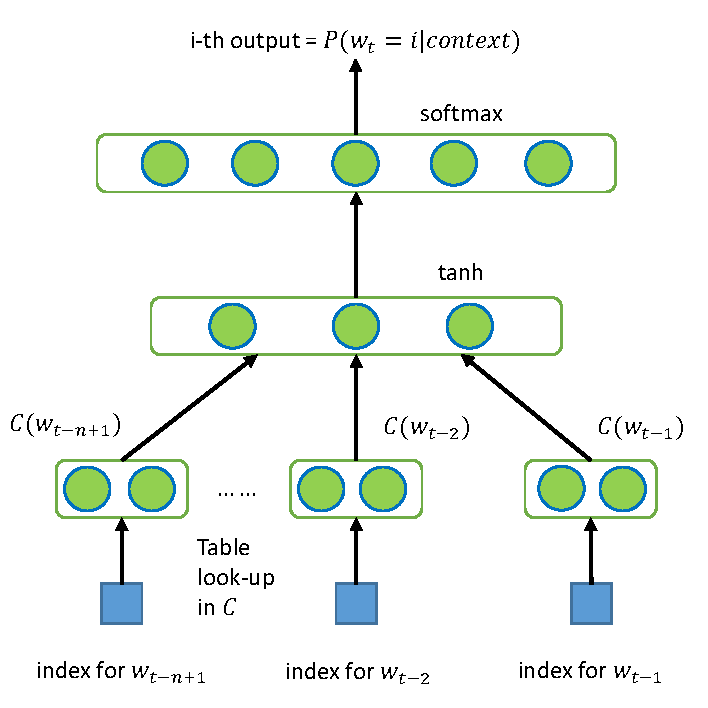
\includegraphics[width= 0.7\textwidth]{figures//nnlm_chap2.pdf}\\
  \caption{神经网络语言模型结构图}\label{fig:nnlm}
\end{figure}

这里主要介绍神经网络语言模型的训练过程如下:

\begin{itemize}
\item 训练数据:一个词序列$w_1, ..., w_T$且任意$w_t \in V$,这里$V$是一个大的有限词汇表。\\
		训练目标:学习一个好的模型$f(w_t, ..., w_{t-n+1}) = \hat{p}(w_t|w_{1}^{t-1})$, 满足对任意$w_{1}^{t-1}$有$\sum_{i=1}^{|V|}f(i, w_{t-1}, ..., w_{t-n+1}) = 1$且$f>0$。
\item 将函数$f(w_t, ..., w_{t-n+1}) = \hat{p}(w_t|w_{1}^{t-1})$分解为两部分:
	\begin{enumerate}
	\item 映射矩阵$C$将$V$中任意元素$i$映射到实数向量$C(i) \in \mathbb{R}^m$,代表词汇表里每一个词的分布式特征向量(distributed feature vector),实际中$C$是一个$|V| \times m$的矩阵。
	\item 基于当前词的概率函数,用$C$来表示:函数$g$将上下文中词序列的特征向量映射为词汇表$V$中下一个词$w_t$出现的条件概率,$g$的输出结果是一个向量,其第$i$个元素估计概率$ \hat{p}(w_t|w_{1}^{t-1})$如图\ref{fig:nnlm}所示。
		\begin{equation}
		f(i, w_i, ..., w_{t-n+1}) = g(i, C(w_{t-1}), ..., C(w_{t-n+1}))
		\end{equation}
	\end{enumerate}
\item 函数$f$是两个映射的组合($C$和$g$),其中$C$在上下文中被所有词所共享。映射$C$中参数时特征向量本身,表示为$|V| \times m$,其中第$i$行$C(i)$是词$i$的特征向量。函数$g$可以由一个前向或者递归神经网络或其他参数函数实现,参数为$\omega $。因此所有的参数集合是$\theta=(C, \omega)$。
\item 参数训练通过求解$\theta$使得训练语料的惩罚log似然最大:
		\begin{equation}
		L=\frac{1}{T}\sum_{t}log(f(w_t,w_{t-1},...,w_{t-n+1};\theta)+R(\theta)
		\end{equation}
		在大多数情况下,神经网络包含一个隐藏层建立在词特征向量映射之上或者直接由词特征向量连接到输出。因此这里实际有两个隐藏层:共享词特征映射层$C$和普通的双曲正切隐藏层。更精确地,神经网络计算如下函数,选用$softmax$输出层保证输出概率值总和为1:
		\begin{equation}
		\hat{p}(w_t|w_{t-1}, ..., w_{t-n+1})=\frac{e^{y_{w_t}}}{\sum_{i}e^{y_i}}
		\end{equation}
		这里$y_i$是每一个输出词$i$的非规范化log概率,通过以下方式来计算,包含参数$b,W,U,d$和$H$:
		\begin{equation}
		y=b+Wx+Utanh(d+Hx)
		\end{equation}
		这里双曲正切tanh逐元的应用,$W$可选置为0(没有从输入词特征向量直接连接到输出层),$x$是词特征层激活向量,通过矩阵$C$中所有输入词特征组合连接而成:
		\begin{equation}
		x=(C(w_{t-1}), C(w_{t-2}), ..., C(w_{t-n+1}))
		\end{equation}
		令$h$作为隐藏单元的个数,$m$作为每个词特征数。当词特征没有直接连接到输出层时,矩阵$W$置为0。则模型的所有自由参数(free parameters)有输出偏置(biases)$b$(包含$|V|$个元素),隐藏层偏置$d$(包含$h$个元素),隐藏层到输出层权重$U$($|V|\times h$矩阵),词特征到输出层权重$W$($|V|\times (n-1)m$矩阵),隐藏层权重$H$($h\times (n-1)m$矩阵)和词特征$C$($|V|\times m$矩阵):
		\begin{equation}
		\theta=(b,d,W,U,H,C)
		\end{equation}
		所有自由参数的总数为$|V|(1+nm+h)+h(1+(n-1)m)$,主要影响因子是$|V|(nm+h)$。
\item 随机梯度下降用来训练该神经网络,通过如下遍历训练语料中第$t$个词的方式迭代更新:
		\begin{equation}
		\theta \leftarrow \theta+\epsilon \frac{\partial log\hat{p}(w_t|w_{t-1}, ..., w_{t-n+1})}{\partial \theta}
		\end{equation}
		这里$\epsilon$是学习率(learning rate)。
\end{itemize}

综上可以看到神经网络语言模型不仅可以学习到词序列即句子的概率值,而且还可以学习到每一个词所对应的特征向量。在文本表示特别是词的表示方法中我们重点关注词特征向量的计算,即矩阵$C$。

%\section{传统词向量表示}

\section{分布式词向量表示}\label{sec_chap2_word2vec}

当前众多的自然语言处理(NLP)系统中,词被视作为原子单元,但是词与词之间的相似度却没有度量,是因为词被表示为词汇表中的下标索引(indices)。通常采用比较流行的N-gram模型用于统计语言模型,如今可以在所有有效数据中来训练N-grams(万亿的词数级别\cite{brants2007large})。但是这类简单方法依赖于大量训练数据,缺失泛化能力。因此在很多任务中都存在缺陷,例如自动语音识别中的领域内数据是有限的;同样地,在机器翻译系统中,大多数语言所有的语料数据也仅仅包含十亿级别的词数或者更少。

随着近年来机器学习技术的进步,依赖大数据来训练更加复杂的模型已经成为可能并且通常效果优于简单模型。特别地,最成功的概念是利用词的分布式表示(distributed representations)\cite{hinton1986learning}。例如,基于语言模型的神经网络模型相比N-gram模型表现更好\cite{bengio2003neural,schwenk2007continuous}。这里强调下分布表示(distributional representations)和分布式表示(distributed representations)的区别。其中分布表示基于共现矩阵,如LSA\cite{landauer1998introduction},PLSA\cite{hofmann1999probabilistic},LDA\cite{blei2003latent}和HAL\cite{lund1996producing}等。而分布式表示则是一个低维、密集、连续值的向量,也称词嵌入式表示(word embeddings)。

因此,Mikolov等人在2013年基于神经网络语言模型提出Word2Vec模型来在大数据集上训练词的分布式向量表示\cite{mikolov2013efficient,mikolov2013distributed,mikolov2013linguistic},包括Continuous Bag-of-Words(CBOW)和Skip-gram两种结构。下面分别简要介绍CBOW和Skip-gram模型:

\begin{figure}[htbp]
  \centering
  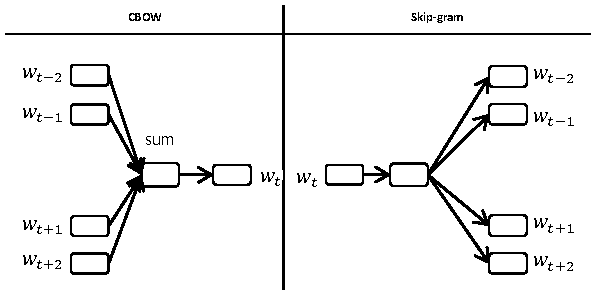
\includegraphics[width= 1.0\textwidth]{figures//word2vec_chap2.pdf}\\
  \caption{Word2Vec结构图}\label{fig:word2vec}
\end{figure}

\begin{itemize}
\item \textbf{CBOW模型}\\
	假设给定词序列$(w_{t-2}, w_{t-1}, w_t, w_{t+1}, w_{t+2})$,其中$w_t$是当前词,其余词作为$w_t$的上下文(context)。如图\ref{fig:word2vec}所示,CBOW模型利用上下文所有词$(w_{t-2}, w_{t-1}, w_{t+1}, w_{t+2})$去预测当前词$w_t$。训练时,给定一个词序列$D=\{w_1, ..., w_M\}$,CBOW模型的学习目标函数定义为最大化如下log似然:
		\begin{equation}\label{eq:cbow}
		{L}_{CBOW}(D)=\frac{1}{M}\sum_{i=1}^{M}\log p(w_{i}|w_{cxt})
		\end{equation}
	这里$w_{cxt}$表示当前词$w_i$的上下文。
\item \textbf{Skip-gram模型}\\
	如图\ref{fig:word2vec}所示,Skip-gram模型利用当前词$w_t$去预测上下文所有词$(w_{t-2}, w_{t-1}, w_{t+1}, w_{t+2})$。训练时,给定一个词序列$D=\{w_1, ..., w_M\}$,Skip-gram模型的学习目标函数定义为最大化如下log似然:
		\begin{equation}\label{eq:skip-gram}
		{L}_{Skip-gram}(D)=\frac{1}{M}\sum_{i=1}^{M}\sum_{-k\leq c\leq k,c\neq 0}\log p(w_{i+c}|w_{i})
		\end{equation}
	这里$k$是上下文窗口大小。
\end{itemize}

另外,在公式\ref{eq:cbow}和\ref{eq:skip-gram}中,对任意变量$w_j$和$w_i$,条件概率$p(w_j|w_i)$通过以下$softmax$函数来计算:
		\begin{equation}\label{eq:softmax}
		p(w_{j}|w_{i})=\frac{\exp(\mathbf{w_{j}} \cdot \mathbf{w_{i}})}{\sum_{w\in W}\exp(\mathbf{w} \cdot \mathbf{w_{i}})}
		\end{equation}

在实际Word2Vec训练中,考虑到$softmax$函数中分母项数量级为$W$,计算$\nabla logp(w_{j}|w_{i})$等比例于$W$,而$W$通常是非常大的($10^5-10^7$词项),因此采用一般的随机梯度下降算法计算代价太大,在实践中并不适用。因此Mikolov等人随机提出了加速$softmax$的算法,包括层次$softmax$(Hierarchical Softmax)和负采样(Negative Sampling)\cite{mikolov2013distributed}。

\begin{itemize}
\item \textbf{层次$softmax$}\\
		层次$softmax$是一个计算高效的$softmax$的近似方法,在神经网络语言模型中,最早由Morin和Bengio提出\cite{morin2005hierarchical}。主要优势是替代原来神经网络中评估$W$个输出节点获得概率分布,层次$softmax$只需评估$log_2(W)$个节点。\\
		层次$softmax$采用一棵以$W$个词作为叶子节点的二叉树,而且对于每一个节点,层次$softmax$明确地表示其子孙节点的相对概率,这定义了一个赋予词以概率值的随机游走过程。\\
		更精确地,每一个词$w$可以由树的根节点通过合适的路径达到。设$n(w,j)$为从根节点root到$w$路径中第$j$个节点,$L(w)$为这个路径的长度。因此$n(w,1)=root$且$n(w,L(w))=w$。另外,对任意的内部节点$n$,设$ch(n)$为一个$n$任意固定的孩子节点且令如果$x$是真,则$\left [ x \right ]$为1,否则为-1。因此层次$softmax$按如下定义$p(w_O|w_I)$:
		\begin{equation}
		p(w|w_I)=\prod_{j=1}^{L(w)-1} \sigma(\left [ n(w,j+1)=ch(n(w,j)) \right ] \cdot {v_{n(w,j)}^{'}}^Tv_{w_I})
		\end{equation}
		这里$\sigma(x)=1/(1+exp(-x))$,可以证明$\sum_{w=1}^{W}p(w|w_I)=1$。这使得$logp(w_O|w_I)$和$\nabla log(w_O|w_I)$的计算代价等比例于$L(w_O)$,$L(w_O)$平均情况不会大于$logW)$。并且,不同于标准$softmax$中每个词$w$被赋予两个表示$v_w$和$v_w^{'}$,而层次$softmax$中每个词$w$只有一个表示$v_w$,并且二叉树中每一个内部节点$n$也有一个表示$v_n^{'}$。\\
		层次$softmax$中树的结构对于性能有着重要的影响,Mnih和Hinton基于对训练时间和结果模型的准确率的考虑探索了很多方法来构造树的结构\cite{mnih2009scalable}。在Word2Vec训练过程中,层次$softmax$采用了霍夫曼树结构,对高频词赋予短的编码来加速训练。因为在实践中观测到提前对词依据出现频率来进行聚簇在神经网络语言模型中是一种非常简单有效的加速技术\cite{mikolov2011extensions,mikolov2013efficient}。
		
\item \textbf{负采样}\\
		层次$softmax$的一种替代方法是噪音对比估计(Noise Contrastive Estimation, NCE),最早由Gutmann和Hycarinen提出\cite{gutmann2012noise}并且由Mnih和Teh用于语言建模中\cite{mnih2012fast}。NCE假设一个好的模型有能力通过逻辑斯蒂回归(logistic regression)从噪音中区分数据,这与Collober和Weston通过对噪音以上的数据进行排序来训练模型所用的hinge损失类似\cite{collobert2008unified}。\\
		NCE可以被证明能够近似最大化$softmax$的log概率,Word2Vec模型仅仅关心学习到高质量的词向量表示,因此可以简化NCE只需保证向量表示的质量即可,按如下方式定义负采样(Negative Sampling):
		\begin{equation}\label{eq:neg}
		log\sigma({v_{w_O}^{'}}^Tv_{w_I})+\sum_{i=1}^{k}E_{w_i}\sim P_{n}(w)\left [log\sigma(-{v_{w_i}^{'}}^Tv_{w_I}\right ]
		\end{equation}
		公式\ref{eq:neg}可以用来替代Word2Vec中的每一个$logP(w_O|w_I)$项。因此,任务变成利用逻辑斯蒂回归(logistic regression)从噪音分布$P_n(w)$区分目标词$w_O$,这里对于每一个数据样本都有$k$个负例样本。实验表明$k$的值范围在5-20之间对于小数据集有利,而对于大数据集,$k$通常设置较小为2-5之间。负采样与NCE之间的主要区别在于NCE同时需要样本和噪音分布的数值概率,而负采样只需要样本。并且NCE目的在于最大化$softmax$的log概率,这个属性对于我们训练向量表示并不重要。
\end{itemize}

相比传统独热表示(one-hot representations)和词袋模型(Bag-of-Words),Word2Vec学习词的分布式向量表示能够更好表征词的特征,泛化能力更强,因此在各项自然语言处理任务中取得最好的结果\cite{mikolov2013efficient,mikolov2013distributed,mikolov2013linguistic,dos2014deep,tang2014learning}。另外,基于Google开源C语言的Word2Vec\footnote{C:https://code.google.com/archive/p/word2vec/},也有多个其他语言版本相继开源如Java\footnote{Java:http://deeplearning4j.org/word2vec}和Python\footnote{Python:https://radimrehurek.com/gensim/models/word2vec.html}等。

受到词的分布式向量表示的启发,研究人员探索新的方法如Pennington等人提出基于全局上下文矩阵分解的Glove模型\cite{pennington2014glove}、基于词的多义现象训练词的多个分布式向量表示\cite{qiu2014co,reisinger2010multi}、融合LDA挖掘词的主题信息来学习词的向量表示解决一词多义的问题\cite{liu2015topical}和更快速的学习词的分布式向量表示的方法\cite{yogatama2014learning,mnih2013learning}。也有基于词向量表示技术扩展至句子、文档\footnote{Doc2Vec:https://radimrehurek.com/gensim/models/doc2vec.html}、词的情感、图结构、文本属性等\cite{le2014distributed,kalchbrenner2014convolutional,tang2014learning,tang2015line,kiros2014multiplicative}。


\section{本章小结}\label{sec_chap2_conclusions}

本章着重介绍本文的背景工作,包括:(1)统计语言模型:简要介绍语言模型的原理与对于自然语言处理任务的意义,并列举了常用的N-gram模型以及其他语言模型;(2)神经网络语言模型:简要介绍神经网络语言模型的由来,重点说明神经网络语言模型的原理;(3)Word2Vec词向量表示:简要介绍了Google基于神经网络语言模型提出Word2Vec模型来学习词的分布式表示,重点介绍Word2Vec的结构包括CBOW和Skip-gram以及训练过程。

本章内容是本文所有工作的基础,基于分布的假设(Distributional Hypotheses)和神经网络语言模型(Neural Network Language Models)来学习文本的分布式表示或向量表示(Distributed Representations or Embedding)的思想贯穿全文,并且训练过程也采用Word2Vec中的随机梯度下降(Stochastic Gradient Descent)以及负采样(Negative Sampling)技术。

%%%%%%%%%%%%%%%%%%
\chapter{学习主题的向量表示}\label{chapter3_topic_representations}

\section{潜在狄利克雷分布}\label{sec_chap3_lda}

潜在狄利克雷分布(Latent Dirichlet Allocation, LDA)\cite{blei2003latent}是一个概率生成模型,LDA假设每篇文档包含多个隐藏主题,而每一个主题则是建立在词汇表里所有词上的一个概率分布。简单来说,LDA按如下方式来生成词序列:

\begin{itemize}
\item 对于文档$d$中第$n$个词$w_n$:
		\begin{itemize}
		\item 采样一个主题$z_n\sim Multinomial(\theta_d)$
		\item 采样一个词$w_n\sim Multinomial(\phi_{z_n})$
		\end{itemize}
\end{itemize}

通常在概率图模型中引入潜在隐藏变量,如LDA中引入隐藏主题(Topics),而采样极大似然估计法(Maximum Likelihood Estimate, MLE)和最大后验概率(Maximum a Posteriori, MAP)来直接推断模型参数会遇到无法直接求导或者计算代价太大的问题\cite{blei2003latent}。因此在实际中通常采用近似推断方法,包括拉普拉斯近似(Laplace approximation)\cite{wolfinger1993laplace}、变分近似(Variational Inference, VI)\cite{jordan1999introduction,wainwright2008graphical}和马尔可夫链蒙特卡洛方法(Markov chain Monte Carlo methods, MCMC)\cite{andrieu2003introduction}等。通过MCMC中最简单的吉布斯采样(Gibbs sampling)\footnote{http://gibbslda.sourceforge.net/},依据当前全条件概率分布( full conditional
distribution)对于每个词进行一定轮数主题采样或至收敛,可以推断学习到文档-主题概率矩阵$\Theta$和主题-词概率矩阵$\Phi$\cite{griffiths2004finding}。依据已有的参数$\Theta$和$\Phi$,可以对任意新来的句子进行同样的采样过程,收敛之后文档中每一个词都会被赋予一个主题。

\section{学习主题向量表示}\label{sec_chap3_topic2vec}

\subsection{研究背景}
依据前面的介绍,我们知道LDA可以挖掘文档中的主题结构信息,而且已经在自然语言处理(NLP)和机器学习(ML)等领域做出巨大的贡献\cite{blei2003latent}。但是,LDA中概率分布仅仅是语料中出现关系的统计结果,并且在实际中,概率分布表示(distrbutional representations)并不是特征表示最好的选择。近来,通过概念以及表示的学习,基于嵌入向量来表示词和文档的方法相继被提出,例如Word2Vec\cite{mikolov2013efficient}和Doc2Vec\cite{le2014distributed}等,而且嵌入向量表示在许多任务中的结果比LDA的概率分布表示更好。

同时,由于词汇表通常在$10^5-10^6$之间,因此LDA还面临严重的长尾现象(long-tail):LDA会赋予语料中的高频词以高概率而低概率的词则很难被选作为主题词。但是在实际中,低概率词有时候可以更好的表征主题。例如,LDA会赋予词$food$高概率并且选为主题词而不是``cheeseburger'',选用高概率词``drug''而不是``aricept'',选用高概率词``technology''而不是``smartphone''。从这些例子可以看出,LDA基于语料的统计结果,会明显偏向于高频词(如``food'',``drugs'',``technology''等),而这些高频词词义通常比较泛,不够具体,不能够非常清晰具体地表征一个主题。相反,部分低频低概率词(如``cheeseburger'',``aricept'',``smartphone''等)词义更加具体,可以更好表征某一个主题。

最近,基于神经网络语言模型(NNLMs)学习的分布式表示将词和文档映射至一个低维的语义向量空间,并且在许多NLP和ML任务中实现了重要的结果\cite{mikolov2013efficient,le2014distributed}。特别地,Word2Vec可以自动学习到词的概念以及词与词之间的语义和句法简单线性关系,例如词向量语义关系:vec(``Berlin'') - vec(``Germany'') = vec(``Paris'') - vec(``France'')和词向量句法关系:vec(``Write'') - vec(``Writing'') = vec(``Read'') - vec(``Reading'')\cite{mikolov2013linguistic}。Doc2Vec在情感分析(Sentiment Analysis)任务中取得了最好的结果\cite{le2014distributed}。自然地,我们会想这个问题:如果将这些主题映射至语义空间将会发生什么?

\subsection{Topic2Vec模型}

受到Word2Vec的启发,我们将主题和词整合到神经网络概率语言模型(NPLM)中。如图\ref{fig:topic2vec}所示,我们提出了Topic2Vec模型能在学习词向量表示的同时学习到主题的向量表示。Topic2Vec同样分为CBOW和Skip-gram两种结构。例如,通过LDA的主题推断,给定一个词-主题序列$(w_{t-2}:z_{t-2}, w_{t-1}:z_{t-1}, w_t:z_t, w_{t+1}:z_{t+1}, w_{t+2}:z_{t+2})$,其中每个词$w_i$都被LDA赋予一个主题$z_i$。通过扩展Word2Vec,在Topic2Vec中,CBOW结构基于上下文词$(w_{t-2}, w_{t-1}, w_{t+1}, w_{t+2})$来预测当前词$w_t$和主题$z_t$,而Skip-gram结构给定当前词$w_t$和主题$z_t$来预测上下文中词$(w_{t-2}, w_{t-1}, w_{t+1}, w_{t+2})$。

\begin{figure}[htbp]
  \centering
  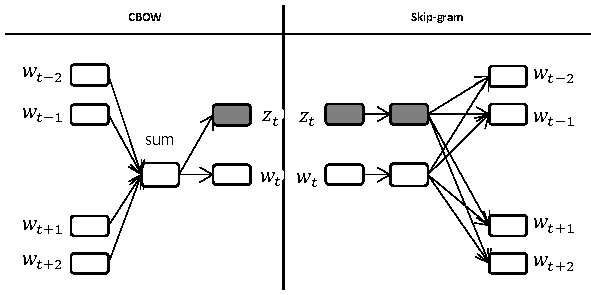
\includegraphics[width= 1.0\textwidth]{figures//topic2vec_chap3.pdf}\\
  \caption{Topic2Vec结构图}\label{fig:topic2vec}
\end{figure}

在Topic2Vec训练之前,需将原始语料数据通过LDA来给语料中每个词赋予一个主题。之后在训练过程中,给定一个文档的词-主题序列$D=\{w_1:z_1, ..., w_M:z_M\}$,其中$z_i$是词$w_i$被LDA所赋予的主题。训练学习目标通过最大如下log似然来定义,分别基于CBOW和Skip-gram模型:

	\begin{equation}
	{L}_{CBOW}(D)=\frac{1}{M}\sum_{i=1}^{M}(\log p(w_{i}|w_{cxt})+\log p(z_{i}|w_{cxt}))
	\end{equation}
	
	\begin{equation}
	{L}_{Skip-gram}(D)=\frac{1}{M}\sum_{i=1}^{M}\sum_{-k\leq c\leq k,c\neq 0}(\log p(w_{i+c}|w_{i})+\log p(w_{i+c}|z_{i}))
	\end{equation}
Topic2Vec模型旨在学习词向量表示的同时能够学习到主题的向量表示。考虑到简单和高效的解决方法,我们沿用了Word2Vec中的优化策略。为了近似最大$softmax$的概率,我们选用负采样(Negative Sampling)而没有用层次$softmax$(Hierarchical Softmax)。随机梯度下降(Stochastic Gredient Descent, SGD)和后向传播(Back-Propagation, BP)算法用来优化我们的模型参数。同时,可以明显看出Topic2Vec模型的复杂度与数据规模呈线性关系,与Word2Vec一致。


\section{实验及分析}\label{sec_chap3}

\subsection{数据集}

\begin{figure}[t]
  \centering
  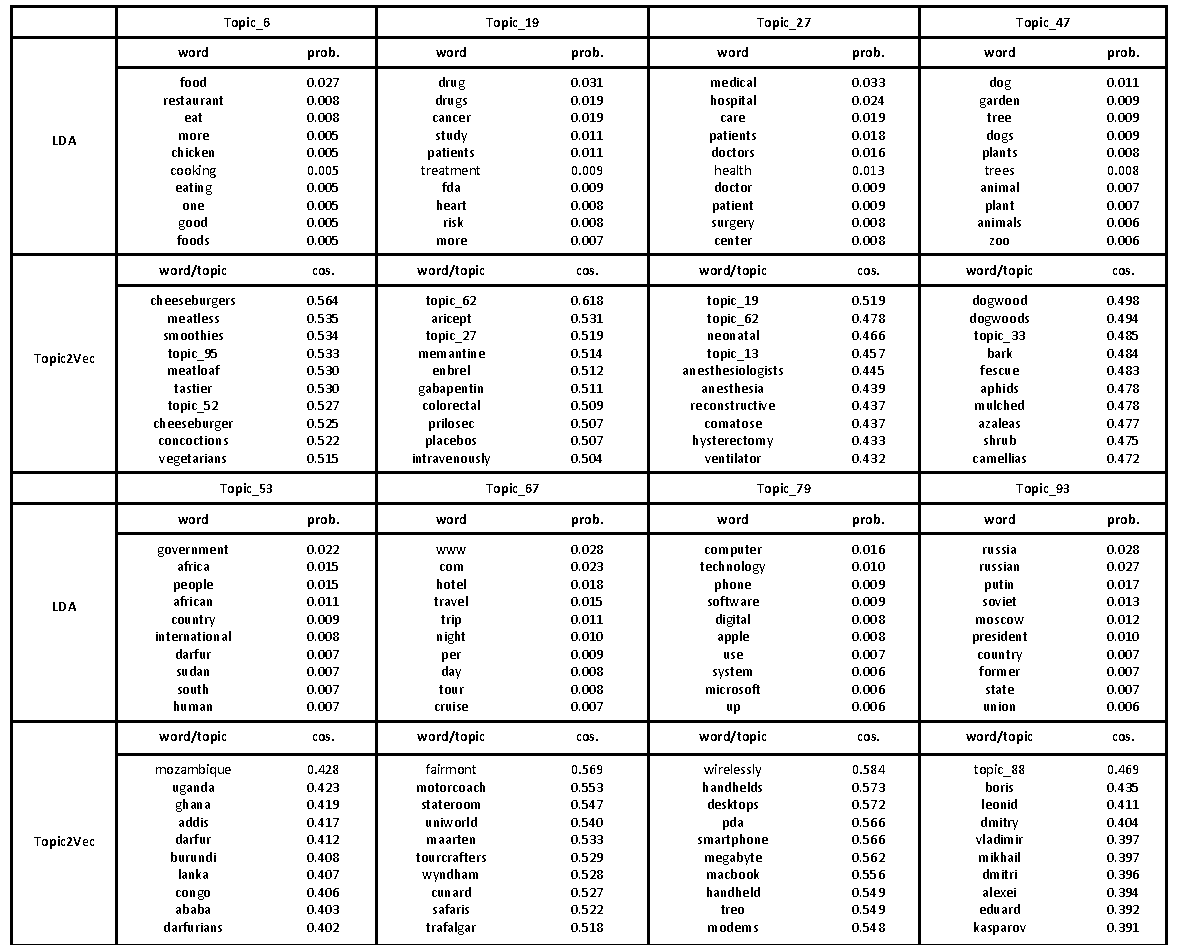
\includegraphics[width= 1.0\textwidth]{figures//topic_words_chap3.pdf}\\
  \caption{对比LDA和Topic2Vec模型列举出给定主题所包含的主题词}\label{fig:topic_words_chap3}
\end{figure}

实验中,我们选用 English Gigaword Fifth Edition\footnote{https://catalog.ldc.upenn.edu/LDC2011T07}作为训练数据来学习词和主题的向量表示。期间我们随机抽取了一定数量的文档来构建训练集如下描述:我们从包含$411032$文档的子目录ltw\_eng(Los Angeles Times)抽取了$100000$文档,其中每一个文档都包含超过$1000$个字符。另外,我们还去除出现次数少于$5$的英文单词和停用词(stop words)。最终,整个训练集包含大约$42000000$个英文单词,词汇表大小为$102644$。

\subsection{评价方法}

\begin{figure}[t]
  \centering
  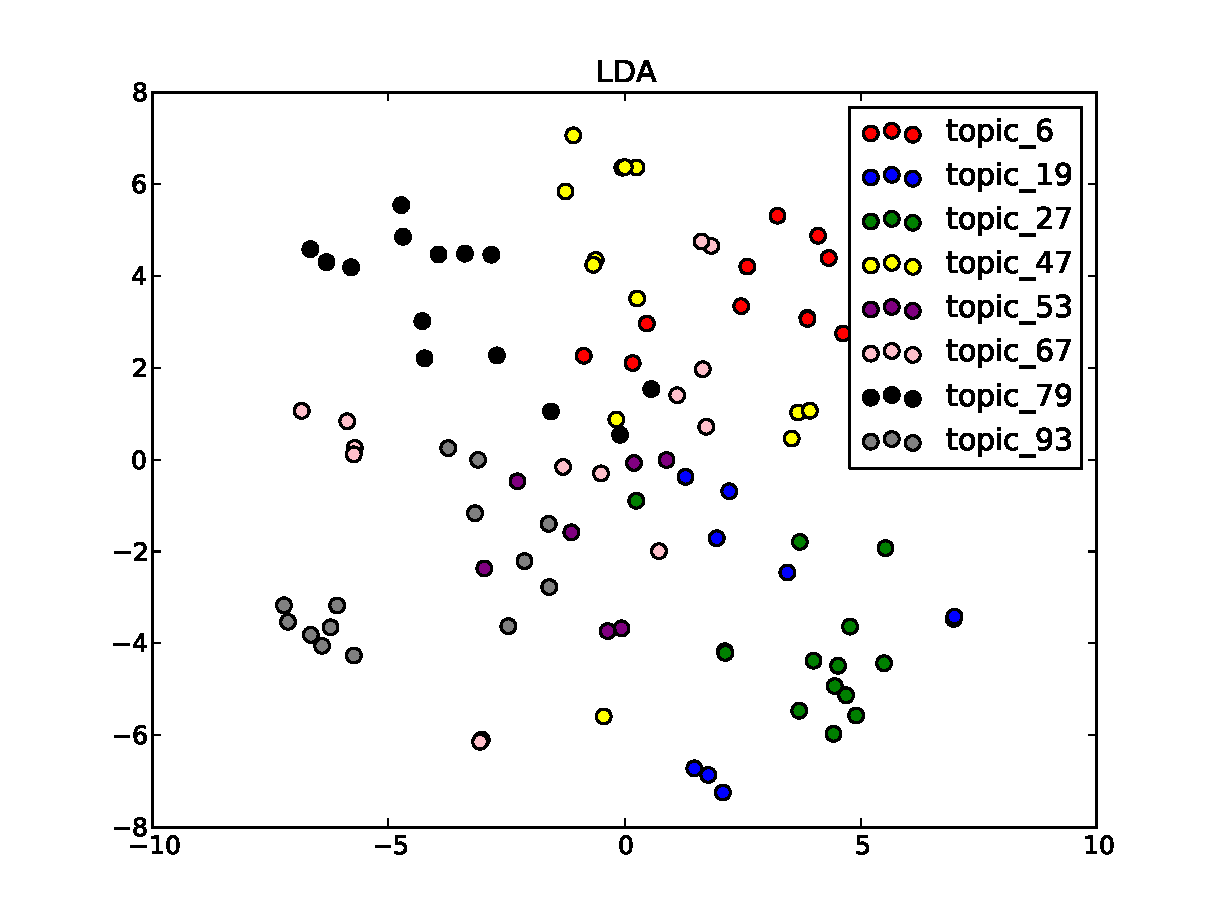
\includegraphics[width= 1.0\textwidth]{figures//lda_tsne_chap3.pdf}\\
  \caption{LDA结果中每个主题所包含主题词基于t-SNE的在2维空间的映射}\label{fig:lda_tsne_chap3}
\end{figure}

在实验中,我们在Skip-gram结构下运行Topic2Vec模型来学习词和主题的分布式向量表示。接着我们将Topic2Vec和原有LDA进行了如下两个方面的对比:(1)我们基于选定的一些主题来选择出每个主题最相关的主题和词;(2)利用t-SNE\cite{van2008visualizing}方法将最相关的主题和词映射至2维空间。在这两个过程中,我们通过如下方式来归纳主题所包含的最相关主题词:

	\begin{itemize}
	\item \textbf{LDA}:每一个主题是所有词的一个概率分布,因此我们依据词与主题之间的条件概率选择最相关的$N=10$个词作为主题词。
	\item \textbf{Topic2Vec}:主题和词被同等地映射至同一个低维的向量空间,因此我们可以通过余弦相似度(cosine similarity)来计算词与主题之间的相似度并且依据相似度来排序选择最相关的主题词。
	\end{itemize}

\subsection{实验结果分析}

\begin{figure}[t]
  \centering
  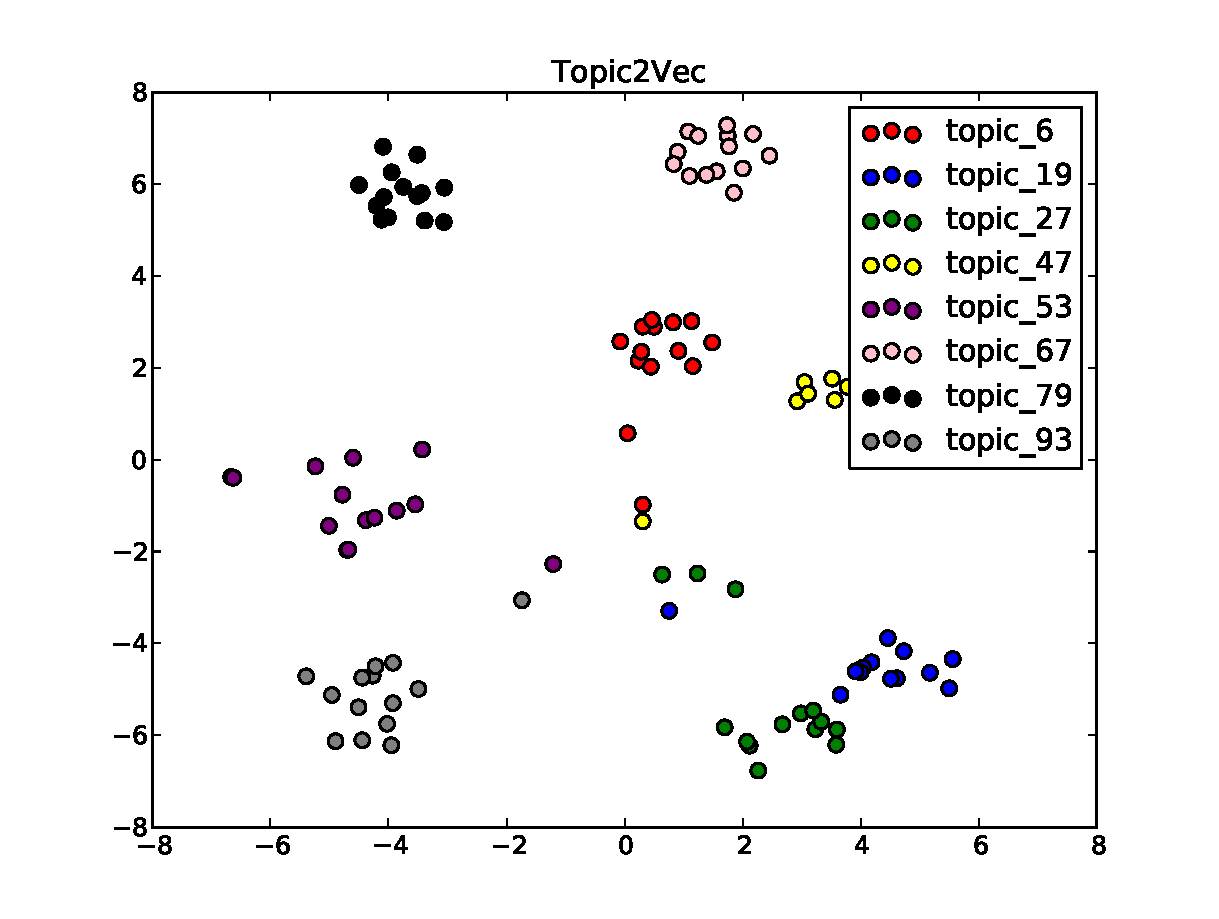
\includegraphics[width= 1.0\textwidth]{figures//tw_tsne_chap3.pdf}\\
  \caption{Topic2Vec结果中每个主题所包含主题和词基于t-SNE的在2维空间的映射}\label{fig:tw_tsne_chap3}
\end{figure}

图\ref{fig:topic_words_chap3}展示出选定8个典型有意义的主题,LDA和Topic2Vec分别给出了最相关的词和主题,我们通过如下细节的分析来理解它们两者之间的不同。如图\ref{fig:topic_words_chap3}所示,对于Topic\_19,LDA返回的主题词如 ``{\it drug}'',``{\it drugs}'',``{\it cancer}''和 ``{\it patients}'',而Topic2Vec返回 ``{\it aricept}'',``{\it memantine}'',``{\it enbrel}''和``{\it gabapentin}'',对于Topic\_27,LDA返回的主题词如 ``{\it medical}'',``{\it hospital}'',``{\it care}'',``{\it patients}''和``{\it doctors}'',而Topic2Vec返回 ``{\it neonatal}'',``{\it anesthesiologists}'',``{\it anesthesia}''和 ``{\it comatose}''。从LDA的结果来看,我们只知道Topic\_19和Topic\_27共享着相同关于``{\it patients}''或者``{\it medical}''的主题,但是我们无法更进一步获得这两个主题之间的不同。但是从Topic2Vec结果来看,我们可以轻易地发现Topic\_19关注一个更加具体的关于药品(``{\it drugs}'')的主题(``{\it aricept}'',``{\it memantine}'',``{\it enbrel}''和``{\it gabapentin}''),而Topic\_27则关注另一个更加具体的关于治疗状况(``{\it treatment}'')的主题(``{\it neonatal}'',``{\it anesthesiologists}'',``{\it anesthesia}''和 ``{\it comatose}''),Topic\_19和Topic\_27本质意义是完全不同的。因此我们得出结论,Topic2Vec在识别两个相似主题时显得更有区别能力。

利用t-SNE降维方法,图\ref{fig:lda_tsne_chap3}和图\ref{fig:tw_tsne_chap3}分别展示出了LDA和Topic2Vec结果的每一个主题所包含最相关主题词在2维空间的映射。明显可以看出,Topic2Vec的结果相同的主题词产生了更好的聚簇而在不同的主题之间产生更好的分离。相反地,LDA并不能产生一个良好分离的映射,不同主题的主题词相互混合在一起。

综上,对于每一个主题而言,Topic2Vec所选定的主题词相比LDA更加具有典型性和代表性。最终,Topic2Vec可以更好的区分不同的主题。

\section{本章小结}\label{sec_chap3_conslusions}

本章首先简要回顾了著名的主题模型潜在狄利克雷分布(LDA),分析了LDA方法中长尾以及概率分布表示存在的问题。之后借鉴Word2Vec基于神经网络语言模型学习词向量表示的思想,将主题和词同时整合到神经网络语言模型中并提出Topic2Vec模型,利用Topic2Vec模型,我们可以将隐藏主题与词映射至同一个语义向量空间。原则上,本章的目的在通过Topic2Vec模型学习新式的嵌入式主题向量表示。另外,通过实验结果的观察,Topic2Vec面对相似的主题相比LDA展示出更强的区别能力。因此,我们可以得出结论:Topic2Vec可以更好的建模主题与词之间的语义关系。

但是目前我们仅仅对于Topic2Vec和LDA进行了定性的评估与分析并且强调了它们二者本质的不同。在未来工作中,我们可以针对二者的不同进行更多细节的定量的分析,包括探索Topic2Vec对于传统自然语言处理任务的提升。

%%%%%%%%%%%%%%%%%%
\chapter{联合学习词及其属性的向量表示}\label{chapter4_word_attributes}

\section{研究背景}

基于我们的认识,词可以表示为词汇表中的下标而文档可以用词袋模型(Bag-of-Words)或N-gram模型来表示。尽管这种表示策略简单高效,但同时也面临众多的不足,例如维度灾难(Curse of Dimensionality)、数据稀疏(Data Sparsity)和缺乏捕获词和文档语义信息(Semantic Information)的能力。

而近来,新式的分布式词向量(Dsitributed Word Representations)表示已经在诸多自然语言处理(NLP)任务中取得重大的成功,例如词性标注(POS-Tagging)、命名实体识别(Name Entity Recognition)和语言建模(Language Modeling)等\cite{bengio2003neural,collobert2008unified,turian2010word,huang2015bidirectional}。另外,分布式表示方法已经被扩展到建模超越词级别的概念,例如短语、句子、文档\cite{le2014distributed},实体与关系\cite{bordes2013translating,socher2013reasoning}、社交和引用网络等\cite{tang2015line}。但是,大多数的模型只利用到局部上下文属性并且单独地学习特定任务相关的表示。因此,这些模型都缺乏可以融合多种属性并利用词及其属性联合学习的能力。

因此在本章,我们提出一个可以同时学习词及其属性的分布式表示的统一框架,其中词的属性可以是词的任意特性。自然地,词属性可以关联到句法关系(词性(POS-Tag)和词元(lemma))、文档结构关系(短语、主题和文档)或者其他信息(例如语言(language)、情感(sentiment)和人名(name of person))。如图\ref{fig:wtld_chap4}中例子所示,词 ``{\it scoring}''具有如下属性:``{\it football}''(主题)、``{\it score}''(词元)和``{\it David Villa opened the scoring. Lionel Messi notched a hat trick. There was also an own goal created by pressure from Messi.}''(文档)。值得注意的是我们可以扩展我们的模型来学习更多词属性的分布式表示,例如``{\it David\ Villa\ opened\ the\ scoring}''(句子)、``{\it positive}''(情感)、``{\it English}''(语言)、``{\it NN}''(词性)和``{\it Lionel\ Messi}''(人名)等。

\begin{figure}[t]
  \centering
  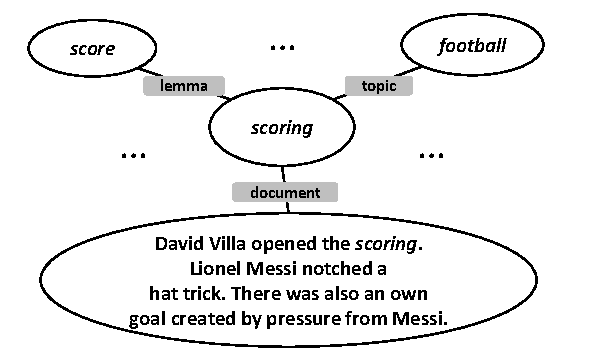
\includegraphics[width= 1.0\textwidth]{figures//word_topic_lemma_document_chap4.pdf}\\
  \caption{词``{\it scoring}''及其节点属性图例}\label{fig:wtld_chap4}
\end{figure}

\begin{table}[t]
\begin{center}
\begin{tabular}{|c|l|l|}
\hline
\textbf{模型} & \multicolumn{1}{c|}{\textbf{词和属性对}} & \multicolumn{1}{c|}{\textbf{学习目标}}                        \\ \hline
Word2Vec        & 词                                              & 词向量表示                                                 \\ \hline
TW              & 词:主题                                        & 主题向量表示与提升的词向量表示 \\ \hline
DW              & 词:文档                                     & 文档向量表示                                            \\ \hline
LW              & 词:词元                                      & 提升的词向量表示                           \\ \hline
TLW             & 词:主题:词元                                 & 提升的词向量表示            \\ \hline
\end{tabular}
\end{center}
\caption{\label{tab:word_attributes} Word2Vec\cite{mikolov2013efficient}和模型(TW, DW, LW and TLW)中所用到词和属性对以及学习目标}
\end{table}

特别地,我们研究了三种词的属性包括主题、词元和文档。基于统一的学习框架,我们提出了四个具体的模型如表\ref{tab:word_attributes}所示:\textbf{TW}整合主题属性来学习分布式主题向量表示,同时可以学习到提升的词向量表示; \textbf{DW}旨在学习分布式文档向量表示; \textbf{LW}整合词元属性来学习提升的词向量表示; \textbf{TLW}则同时整合主题和词元属性来提升词向量表示。总结我们本章的工作如下:

\begin{itemize}
\item 我们提出了一个学习词和属性分布式表示的统一框架,见\ref{subsec_unifiedfk_chap4}。
\item 基于统一的学习框架,我们提出的模型可以学习主题(见\ref{subsec_tw_chap4})和文档(见\ref{subsec_dw_chap4})的分布式表示。
\item 我们提出的模型(TW, LW和TLW)可以利用额外的属性(主题和词元)来提升词的向量表示((见\ref{subsec_improved_we_chap4}))。
\end{itemize}

实验结果表明我们的模型不仅可以对于特定任务学习到属性表示,而且可以利用额外的属性知识来提升词的向量表示。


\section{框架与模型}\label{sec_our_models_chap4}

\subsection{联合学习词和属性向量表示的统一框架}\label{subsec_unifiedfk_chap4}

借鉴神经网络语言模型(NPLMs)和Word2Vec模型,我们提出了一个联合学习词和属性分布式向量表示的统一学习框架,如图\ref{fig:ourfk_chap4}(c)和(d)所示。例如给定一个词序列$(w_{t-2}, w_{t-1}, w_t, w_{t+1}, w_{t+2})$,其中$w_t$是当前词并且被赋予$k$个属性$(a_{t,1}, ..., a_{t,k})$,CBOW模型如图\ref{fig:ourfk_chap4}(c)所示,基于上下文词$(w_{t-2}, w_{t-1}, w_{t+1}, w_{t+2})$来预测当前词$w_t$和$k$个属性$(a_{t,1}, ..., a_{t,k})$,而Skip-gram模型给定当前词$w_t$和$k$个属性$(a_{t,1}, ..., a_{t,k})$来预测上下文词$(w_{t-2}, w_{t-1}, w_t, w_{t+1}, w_{t+2})$。

\begin{figure}[htbp]
  \centering
  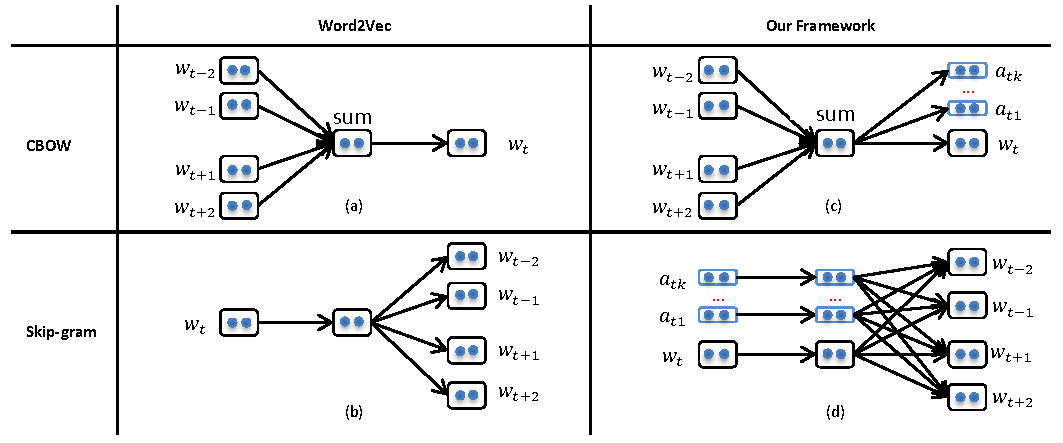
\includegraphics[width= 1.0\textwidth]{figures//our_framework_chap4.pdf}\\
  \caption{Word2Vec和统一学习框架中的CBOW和Skip-gram模型结构对比图}\label{fig:ourfk_chap4}
\end{figure}

基于我们提出的框架模型,可以明显地看出词和属性在学习过程中可以相互帮助提升来得到更好的向量表示。

特别地,在本章我们考虑了三种属性:主题、词元和文档并分别提出了相应的模型TW、DW、LW和TLW。基于Harris及后来Pantel等人提出的词分布假设(distributional hypothesis)\cite{harris1954distributional,pantel2005inducing},我们假设词属性也具有相似的分布假设。而且我们的模型也受到如下分布假设的驱动:

\begin{itemize}
\item \textbf{Hypothesis A}: {\em 出现在相同上下文中的词具有相似的意义。( ``words that occur in the same contexts tend to have similar meanings" (Pantel, 2005))}.
\item \textbf{Hypothesis B}: {\em 出现在相同上下文中的词所赋予的主题也是相似的。(``topics assigned to words that occur in the same contexts tend to be similar")}.
\item \textbf{Hypothesis C}: {\em 出现在相同上下文中的词所属的词元也是相似的。(``lemmas of words that occur in the same contexts tend to be similar")}.
\item \textbf{Hypothesis D}: {\em 出现在相同上下文中的词所属的文档也是相似的。(``documents consisting of words that occur in the same contexts tend to be similar")}.
\end{itemize}

\subsection{TW模型:学习主题向量表示}\label{subsec_tw_chap4}

如表\ref{tab:word_attributes}所示,TW考虑了词所赋予的主题属性旨在学习分布式主题向量表示。例如给定一个词-主题序列$(w_{t-2}:z_{t-2}, w_{t-1}:z_{t-1}, w_t:z_t, w_{t+1}:z_{t+1}, w_{t+2}:z_{t+2})$,其中$w_t$是当前词并伴随着一个从$GibbsLDA++$\footnote{http://gibbslda.sourceforge.net/}学到的主题属性$z_t$,CBOW模型基于上下文词$(w_{t-2}, w_{t-1}, w_{t+1}, w_{t+2})$来预测当前词$w_t$和主题$z_t$,而Skip-gram模型给定当前词$w_t$和主题$z_t$来预测上下文词$(w_{t-2}, w_{t-1}, w_{t+1}, w_{t+2})$。

当开始训练时,给定一个词-主题序列$D=\left \{w_{1}:z_{1},...,w_{M}:z_{M}  \right \}$,学习目标通过最大如下log似然来定义,分别基于CBOW和Skip-gram模型:

	\begin{equation}\label{eq:tw_cbow_chap4}
	{L}_{CBOW}(D)=\frac{1}{M}\sum_{i=1}^{M}(\log p(w_{i}|w_{cxt})+\log p(z_{i}|w_{cxt}))
	\end{equation}
	
	\begin{equation}\label{eq:tw_skip-gram_chap4}
	{L}_{Skip-gram}(D)=\frac{1}{M}\sum_{i=1}^{M}\sum_{-k\leq c\leq k,c\neq 0}(\log p(w_{i+c}|w_{i})+\log p(w_{i+c}|z_{i}))
	\end{equation}

值得注意的是,在上述公式\ref{eq:tw_cbow_chap4}和公式\ref{eq:tw_skip-gram_chap4}中,第一部分关于$w_i$基于\textbf{Hypothesis A}而第二部分关于$z_i$基于\textbf{Hypothesis B}。不同于传统LDA中作为一个在词表上的概率分布的主题表示方法,TW模型将词和主题属性映射至同一个语义空间。在相同的语义空间里,词和主题的相似度可以直接采用余弦函数来计算。

\subsection{DW模型:学习文档向量表示}\label{subsec_dw_chap4}

如表\ref{tab:word_attributes}所示,DW考虑了词所赋予的文档属性旨在学习分布式文档向量表示。例如给定一个词-文档序列$(w_{t-2}:d_{t-2}, w_{t-1}:d_{t-1}, w_t:d_t, w_{t+1}:d_{t+1}, w_{t+2}:d_{t+2})$,其中$w_t$是当前词并伴随着一个包含这个词的文档属性$d_t$,CBOW模型基于上下文词$(w_{t-2}, w_{t-1}, w_{t+1}, w_{t+2})$来预测当前词$w_t$和文档$d_t$,而Skip-gram模型给定当前词$w_t$和文档$d_t$来预测上下文词$(w_{t-2}, w_{t-1}, w_{t+1}, w_{t+2})$。

当开始训练时,给定一个词-文档序列$D=\left \{w_{1}:d_{1},...,w_{M}:d_{M}  \right \}$,学习目标通过最大如下log似然来定义,分别基于CBOW和Skip-gram模型:

	\begin{equation}\label{eq:dw_cbow_chap4}
	{L}_{CBOW}(D)=\frac{1}{M}\sum_{i=1}^{M}(\log p(w_{i}|w_{cxt})+\log p(d_{i}|w_{cxt}))
	\end{equation}
	
	\begin{equation}\label{eq:dw_skip-gram_chap4}
	{L}_{Skip-gram}(D)=\frac{1}{M}\sum_{i=1}^{M}\sum_{-k\leq c\leq k,c\neq 0}(\log p(w_{i+c}|w_{i})+\log p(w_{i+c}|d_{i}))
	\end{equation}

值得注意的是,在上述公式\ref{eq:dw_cbow_chap4}和公式\ref{eq:dw_skip-gram_chap4}中,第一部分关于$w_i$基于\textbf{Hypothesis A}而第二部分关于$d_i$基于\textbf{Hypothesis D}。文档作为词的属性导致了包含在同一个文档中的所有词更难于区别,因此DW模型使得词的向量表示更差。因此在本文中,DW仅仅关注与学习文档的分布式表示而不能够提升词的向量表示。

\subsection{提升词向量表示的模型}\label{subsec_improved_we_chap4}

\begin{figure}[htbp]
  \centering
  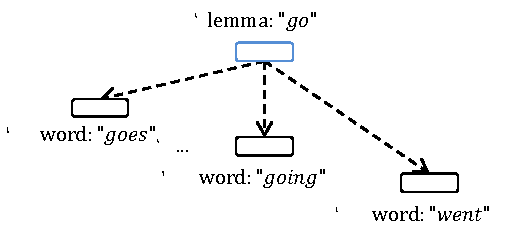
\includegraphics[width= 1.0\textwidth]{figures//lemma_word_chap4.pdf}\\
  \caption{形态学中一个词元及其变种词的例子}\label{fig:lemma_word_chap4}
\end{figure}

\begin{itemize}
\item \textbf{TW} 如前面在\ref{subsec_tw_chap4}中描述,TW模型可以联合学习词向量表示和分布式主题向量表示。同只利用到局部上下文的Word2Vec模型相比,TW模型同时考虑了词和主题属性。自然地,我们期望运用额外的主题属性可以提升原来的词向量表示。

\item \textbf{LW} 在形态学(Morphology)中,词元(Lemma)\footnote{https://en.wikipedia.org/wiki/Lemma}是一组词的规范化(canonical)形式。在英语中,例如单词``{\it go}'',``{\it goes}'',``{\it went}''和``{\it going}''是同一个词素(Lexeme)的不同形式,以单词``{\it go}''作为词元,如图\ref{fig:lemma_word_chap4}所示。拥有相同词元的不同单词通常包含着相同的基本意义。

如表\ref{tab:word_attributes}所示,LW考虑了词所赋予的词元属性旨在提升词的向量表示。例如给定一个词-词元序列$(w_{t-2}:l_{t-2}, w_{t-1}:l_{t-1}, w_t:l_t, w_{t+1}:l_{t+1}, w_{t+2}:l_{t+2})$,其中$w_t$是当前词并伴随着一个由$WordNet\ Lemmatizer$\footnote{http://textanalysisonline.com/nltk-wordnet-lemmatizer}获取的词元属性$l_t$,CBOW模型基于上下文词$(w_{t-2}, w_{t-1}, w_{t+1}, w_{t+2})$来预测当前词$w_t$和词元$l_t$,而Skip-gram模型给定当前词$w_t$和词元$l_t$来预测上下文词$(w_{t-2}, w_{t-1}, w_{t+1}, w_{t+2})$。

当开始训练时,给定一个词-词元序列$D=\left \{w_{1}:l_{1},...,w_{M}:l_{M}  \right \}$,学习目标通过最大如下log似然来定义,分别基于CBOW和Skip-gram模型:

	\begin{equation}\label{eq:lw_cbow_chap4}
	{L}_{CBOW}(D)=\frac{1}{M}\sum_{i=1}^{M}(\log p(w_{i}|w_{cxt})+\log p(l_{i}|w_{cxt}))
	\end{equation}
	
	\begin{equation}\label{eq:lw_skip-gram_chap4}
	{L}_{Skip-gram}(D)=\frac{1}{M}\sum_{i=1}^{M}\sum_{-k\leq c\leq k,c\neq 0}(\log p(w_{i+c}|w_{i})+\log p(w_{i+c}|l_{i}))
	\end{equation}

值得注意的是,在上述公式\ref{eq:lw_cbow_chap4}和公式\ref{eq:lw_skip-gram_chap4}中,第一部分关于$w_i$基于\textbf{Hypothesis A}而第二部分关于$l_i$基于\textbf{Hypothesis C}。

\item \textbf{TLW} 如表\ref{tab:word_attributes}所示,TLW同时考虑了词所赋予的主题和词元属性旨在提升词的向量表示。例如给定一个词-主题-词元序列$(w_{t-2}:z_{t-2}:l_{t-2},w_{t-1}:z_{t-1}:l_{t-1},w_{t}:z_{t}:l_{t},w_{t+1}:z_{t+1}:l_{t+1},w_{t+2}:z_{t+2}:l_{t+2})$,其中$w_t$是当前词并伴随着一个主题属性$z_t$和一个词元属性$l_t$,CBOW模型基于上下文词$(w_{t-2}, w_{t-1}, w_{t+1}, w_{t+2})$来预测当前词$w_t$、主题$z_t$和词元$l_t$,而Skip-gram模型给定当前词$w_t$、主题$z_t$和词元$l_t$来预测上下文词$(w_{t-2}, w_{t-1}, w_{t+1}, w_{t+2})$。

当开始训练时,给定一个词-词元序列$D=\left \{w_{1}:z_{1}:l_{1},...,w_{M}:z_{M}:l_{M}  \right \}$,学习目标通过最大如下log似然来定义,分别基于CBOW和Skip-gram模型:

	\begin{equation}\label{eq:tlw_cbow_chap4}
	{L}_{CBOW}(D)=\frac{1}{M}\sum_{i=1}^{M}(\log p(w_{i}|w_{cxt})+\log p(z_{i}|w_{cxt})+\log p(l_{i}|w_{cxt}))
	\end{equation}
	
	\begin{equation}\label{eq:tlw_skip-gram_chap4}
	{L}_{Skip-gram}(D)=\frac{1}{M}\sum_{i=1}^{M}\sum_{-k\leq c\leq k,c\neq 0}(\log p(w_{i+c}|w_{i})+\log p(w_{i+c}|z_{i})+\log p(w_{i+c}|l_{i}))
	\end{equation}

值得注意的是,在上述公式\ref{eq:tlw_cbow_chap4}和公式\ref{eq:tlw_skip-gram_chap4}中,第一部分关于$w_i$基于\textbf{Hypothesis A},第二部分关于$z_i$是基于\textbf{Hypothesis B},而第三部分关于$l_i$基于\textbf{Hypothesis C}。

\end{itemize}

\subsection{优化和学习过程}\label{subsec_optimize_chap4}

同样地,考虑到简单和高效的解决方法,我们沿用了Word2Vec中的优化策略。为了近似最大$softmax$的log概率,我们选用负采样(Negative Sampling)而没有用层次$softmax$(Hierarchical Softmax)\cite{mikolov2013distributed}。随机梯度下降(Stochastic Gredient Descent, SGD)和后向传播(Back-Propagation, BP)算法用来优化我们的模型参数。

特别地,TW模型集中来学习主题的分布式向量表示,而DW则学习文档的分布式向量表示。更甚者,TW、LW和TLW模型可以提升词向量表示。在具体实现中,这些模型首先初始化词和主题等属性的向量表示,然后联合的学习各自的分布式表示。而对于DW,我们仅仅对文档向量进行了随机初始化,对于词向量采用了预先从大规模和高质量的数据集中学习到的词向量来初始化,然后DW模型来学习文档的分布式表示,并且保持词向量表示不变。由我们模型的学习目标函数可以明显看出,模型的复杂度与数据集呈线性关系,与Word2Vec保持一致。

\section{实验及分析}\label{sec_exps_chap4}

\subsection{数据集}\label{subsec_datasets_chap4}

\begin{figure}[t]
  \centering
  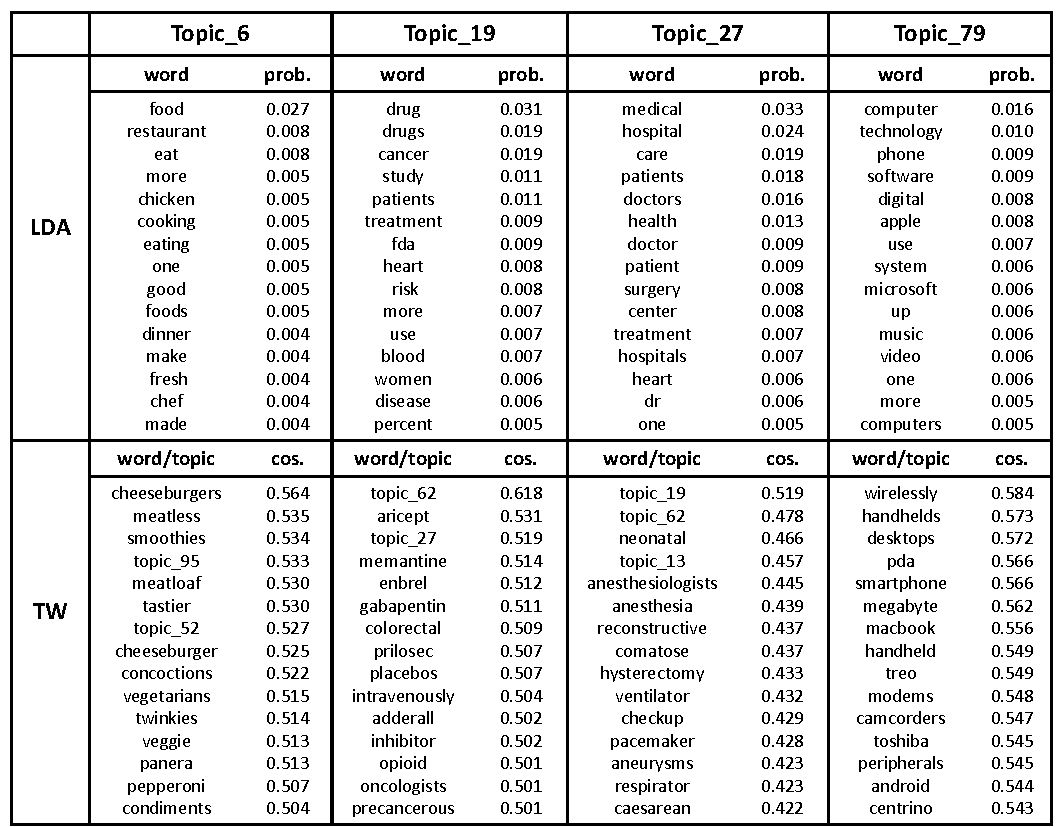
\includegraphics[width= 1.0\textwidth]{figures//topic_words_chap4.pdf}\\
  \caption{对比LDA和TW模型列举出给定主题所包含的主题词}\label{fig:topic_words_chap4}
\end{figure}

我们选用英语Gigaword\footnote{https://catalog.ldc.upenn.edu/LDC2011T07}作为训练数据来学习基础词向量表示。实际中,我们随机选择了一些文档并且按如下方式构造了两个不同大小的训练集:

\begin{itemize}
\item \textbf{DS-100k}:我们从包含了$411032$文档数的子目录ltw\_eng(Los Angeles Times)中选取了$100000$的文档,每个文档至少包含$1000$个字符。另外,我们去除掉出现次数少于$5$的词和停用词(stop words)。最终,DS-100k数据集包含$42000000$的单词而整个词汇表的大小为$102644$。
\item \textbf{DS-500k}:我们还从包含了$1962178$文档数的子目录nyt\_eng(New York Times)中选取了$500000$的文档。在去除出现次数少于$5$的单词和停用词之后,DS-500k最终大约包含了$2.1$亿的单词而整个词汇表的大小为$232481$。
\end{itemize}
另外,我们在数据集DS-100k上运行了$GibbsLDA++$和TW模型来评估主题的向量表示,并且在$20NewsGroup$\footnote{http://qwone.com/~jason/20Newsgroups/}上进行了文档向量表示的评估。

\subsection{评估主题向量表示}\label{subsec_evaluate_topic_chap4}

\begin{figure}[htbp]
  \centering
  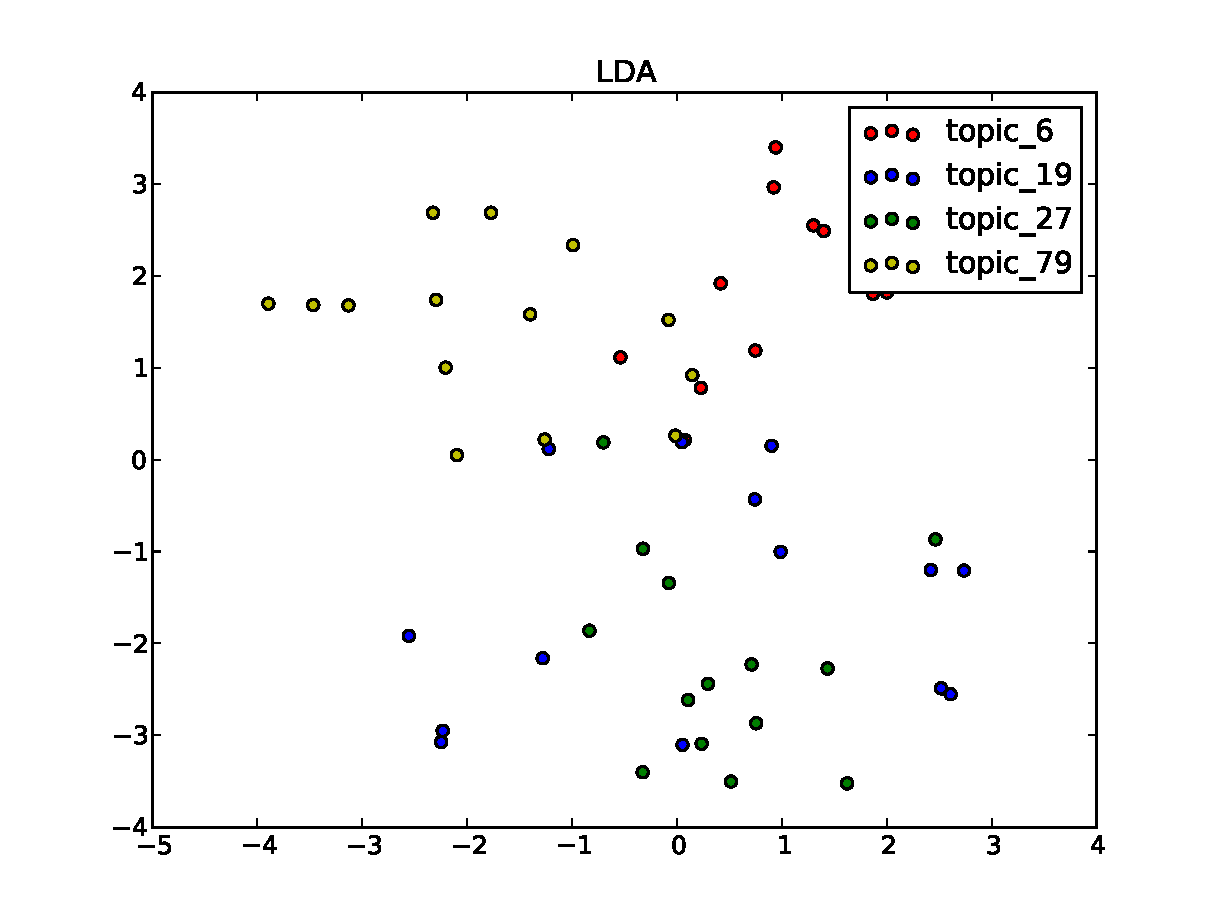
\includegraphics[width= 1.0\textwidth]{figures//lda_tsne_chap4.pdf}\\
  \caption{LDA结果中每个主题所包含主题词基于t-SNE的在2维空间的映射}\label{fig:lda_tsne_chap4}
\end{figure}

TW模型能够在学习词向量表示的同时学习主题的向量表示。因此我们首先进行实验与原始LDA\cite{blei2003latent}模型来对比评估TW模型学习到的主题向量表示。我们按照如下方式来选取主题所包含的主题词:

	\begin{itemize}
	\item \textbf{LDA}:所有的主题都表示为词汇表上的概率分布,因此我们依据词与主题之间的条件概率选择最相关的$N=15$个词作为主题词。
	\item \textbf{TW}:所有的主题和词被同等地映射至同一个低维的向量空间,因此我们可以通过余弦相似度(cosine similarity)来计算词与主题之间的相似度并且依据相似度来排序选择最相关的主题词。
	\end{itemize}
	
\begin{figure}[htbp]
\centering
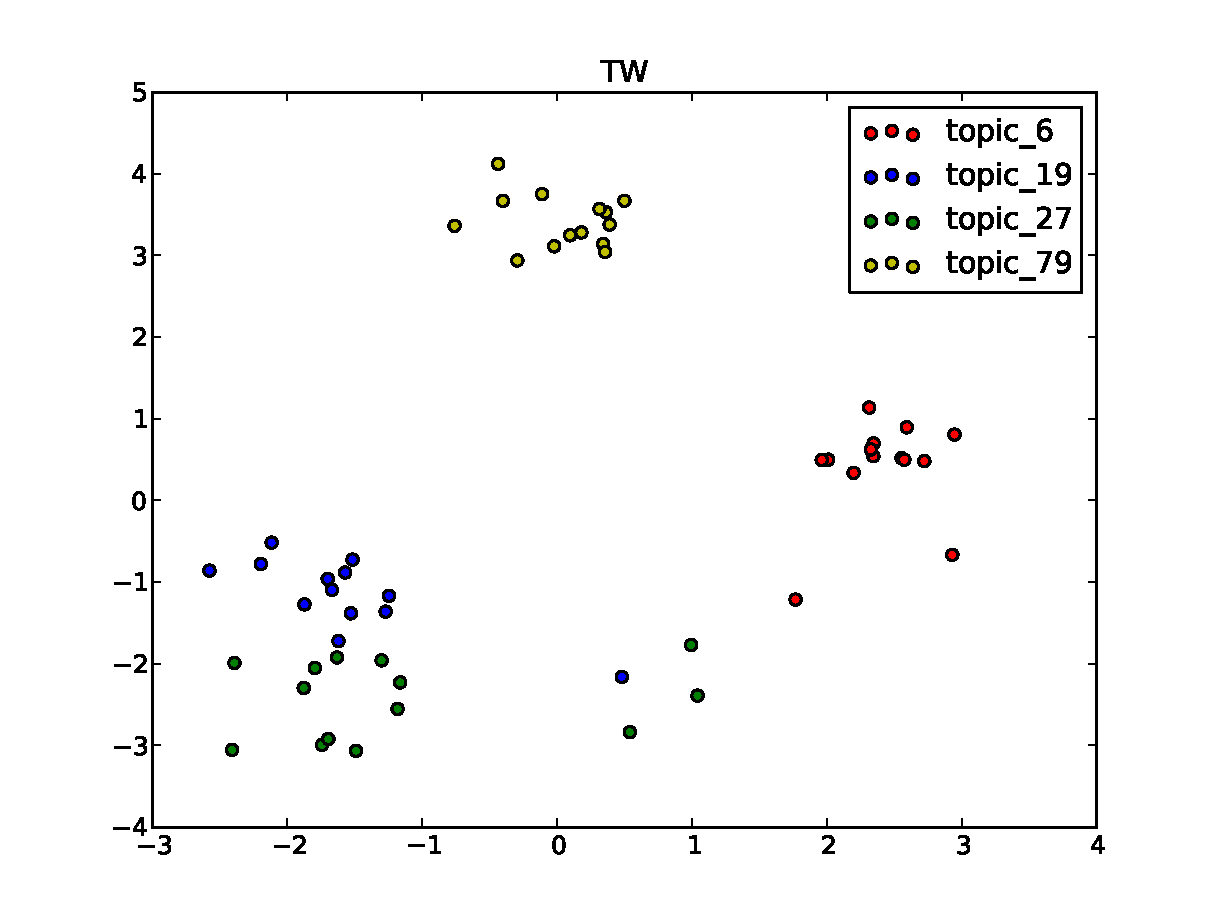
\includegraphics[width= 1.0\textwidth]{figures//tw_tsne_chap4.pdf}\\
\caption{TW结果中每个主题所包含主题词基于t-SNE的在2维空间的映射}\label{fig:tw_tsne_chap4}
\end{figure}
	
图\ref{fig:topic_words_chap4}展示出选定4个典型有意义的主题,LDA和TW分别给出了最相关的词和主题,我们通过如下细节的分析来理解它们两者之间的不同。
如图\ref{fig:topic_words_chap4}所示,对于Topic\_19,LDA返回的主题词如 ``{\it drug}'',``{\it drugs}'',``{\it cancer}''和 ``{\it patients}'',而TW返回 ``{\it aricept}'',``{\it memantine}'',``{\it enbrel}''和``{\it gabapentin}'',对于Topic\_27,LDA返回的主题词如 ``{\it medical}'',``{\it hospital}'',``{\it care}'',``{\it patients}''和``{\it doctors}'',而TW返回 ``{\it neonatal}'',``{\it anesthesiologists}'',``{\it anesthesia}''和 ``{\it comatose}''。从LDA的结果来看,我们只知道Topic\_19和Topic\_27共享着相同关于``{\it patients}''或者``{\it medical}''的主题,但是我们无法更进一步获得这两个主题之间的不同。但是从TW结果来看,我们可以轻易地发现Topic\_19关注一个更加具体的关于药品(``{\it drugs}'')的主题(``{\it aricept}'',``{\it memantine}'',``{\it enbrel}''和``{\it gabapentin}''),而Topic\_27则关注另一个更加具体的关于治疗状况(``{\it treatment}'')的主题(``{\it neonatal}'',``{\it anesthesiologists}'',``{\it anesthesia}''和 ``{\it comatose}''),Topic\_19和Topic\_27本质意义是完全不同的。明显地可以看出TW在识别两个相似主题时显得更有区别能力。

利用t-SNE\cite{van2008visualizing}降维方法,图\ref{fig:lda_tsne_chap4}和图\ref{fig:tw_tsne_chap4}分别展示出了LDA和TW结果的每一个主题所包含最相关主题词在2维空间的映射。明显可以看出,TW的结果相同的主题词产生了更好的聚簇而在不同的主题之间产生更好的分离。相反地,LDA并不能产生一个良好分离的映射,不同主题的主题词相互混合在一起。

综上,对于每一个主题而言,TW所选定的主题词相比LDA更加具有典型性和代表性。最终,TW可以更好的区分不同的主题。

\subsection{评估文档向量表示}\label{subsec_evaluate_doc_chap4}

\begin{itemize}
\item \textbf{文本分类(Text Classification)} DW集中学习文档的分布式向量表示,因此我们通过多分类(Multi-Class)的文本分类任务来评估文档向量表示。我们选用标准的$20NewsGroup$数据集,其中包含了从$20$个不同的新闻组收集到的大约$20000$的文档。考虑到$20NewsGroup$数据集对于训练词向量表示时数据不足的问题,我们首先基于大数据集DS-500k来训练得到词的向量表示。然后DW模型开始学习$20NewsGroup$中的文档的向量表示,并且保持词向量表示不变。

\end{itemize}

\begin{table}[htbp]
\centering
\begin{tabular}{|c|c|c|c|c|c|c|}
\hline
\multicolumn{2}{|c|}{模型}                                                                                                           & 维度                                                    & 准确率                                                   & 精确度                                                  & 回归率                                                     & F1度量                                                  \\ \hline
\multicolumn{2}{|c|}{\begin{tabular}[c]{@{}c@{}}LDA\\ PV-DM\\ PV-DBOW\end{tabular}} & \begin{tabular}[c]{@{}c@{}}80\\ 400\\ 400\end{tabular} & \begin{tabular}[c]{@{}c@{}}72.2\\ 72.4\\ 75.4\end{tabular} & \begin{tabular}[c]{@{}c@{}}70.8\\ 72.1\\ 74.9\end{tabular} & \begin{tabular}[c]{@{}c@{}}70.7\\ 71.5\\ 74.3\end{tabular} & \begin{tabular}[c]{@{}c@{}}70.0\\ 71.5\\ 74.3\end{tabular} \\ \hline
\multirow{4}{*}{DW}                  & \multirow{2}{*}{CBOW}             & 300                                                    & 74.4                                                       & 73.9                                                       & 73.5                                                       & 73.4                                                       \\ \cline{3-7} 
                                      &                                   & 400                                                    &\textbf{75.8}                                                            &\textbf{75.4}                                           &\textbf{74.9}                                                            &\textbf{74.8}                                                            \\ \cline{2-7} 
                                      & \multirow{2}{*}{Skip-gram}        & 300                                                    & 72.1                                                       & 71.5                                                       & 71.2                                                       & 71.1                                                       \\ \cline{3-7} 
                                      &                                   & 400                                                    &72.9                                                        & 72.4                                                        &72.1                                                        & 72.2                                                         \\ \hline
\end{tabular}
\caption{DW模型与其他模型在$20NewsGroup$数据集上的实验对比。其他方法的结果见\cite{liu2015topical}。粗体表示所有结果中最好的结果。}
\label{tab:tc_chap4}
\end{table}

对于每一个文档,DW返回一个对应的向量作为这个文档的表示。紧接着我们利用采用了``一对剩余所有''(``one vs rest'')模式的LIBLINEAR\footnote{http://www.csie.ntu.edu.tw/~cjlin/liblinear/} 来做多类别的文本分类。为了评价我们模型的有效性,我们将DW模型与其他学习文档表示的模型进行了实验对比,包括LDA以及最近提出的段落向量表示模型(Paragraph Vector Model)\cite{le2014distributed}。其中,LDA将每个文档表示为隐藏主题上的概率分布,而段落向量表示模型则将每个文档表示为一个低维的连续向量,包括分布式记忆模型(distributed memory model, PV-DM)和分布式词袋模型(distributed bag-of-words model, PV-DBOW)。如表\ref{tab:tc_chap4}所示,DW模型相比已有模型实现了具有竞争力的结果。值得注意的是,所有这些学习文档的低维连续值向量表示的方法的性能都不如传统的词袋模型(BOW)和TWE-1模型\cite{liu2015topical},其中后两者方法均利用了语料数据的TF-IDF特征来帮助文本分类。


\subsection{评估提升的词向量表示}\label{subsec_evaluate_improved_word_chap4}

最终我们通过如下的标准任务来评估提升的词向量表示:

\begin{itemize}
\item \textbf{词类比(Word Analogy)} 实验中采用两个数据集用于这个任务。其中谷歌数据集\cite{mikolov2013distributed}包含$10675$个句法问题(如{\em young:yonger::large:larger})和$8869$个语义问题(如{\em Rome:Italy::Athens:Greece})。微软数据集\cite{mikolov2013linguistic}\footnote{http://research.microsoft.com/enus/projects/rnn/default.aspx}包含了$8000$个句法问题(如{\em good:better::rough:rougher})。在每一个问题中,第四个单词是缺失的,而这个任务是正确地预测第四个单词。我们采用向量偏移(vector offset)方法\cite{mikolov2013distributed}来计算第四个单词的向量表示$\mathbf{w_{fourth}}=\mathbf{w_{third}}+(\mathbf{w_{second}}-\mathbf{w_{first}})$,如果向量$\mathbf{w_{fourth}}$与正确答案的向量具有最高的余弦相似度,则这个问题算作回答正确。

我们通过将我们的模型与基准模型Word2Vec\cite{mikolov2013efficient}和目前最好的模型Glove\cite{pennington2014glove}\footnote{http://nlp.stanford.edu/projects/glove/}进行了结果对比。如表\ref{tab:wordanalogies_chap4}所示,LW和TLW模型相比Word2Vec在多数Skip-gram情况下表现更好,而TW不能。原有似乎是词元信息在词类比这个任务中相比主题信息可以获得更多的提升。更准确地,在DS-100k数据集上和Skip-gram情况下,TLW在谷歌语义上提升了+8.48\%而LW在微软句法上提升了+5.57\%。在更大的DS-500k数据集上和Skip-gram情况下,LW在谷歌语义问题上提升了+3.95\%而在微软句法问题上提升了+2.72\%。一般地,我们可以得出如下的结论:

	\begin{itemize}
	\item 在词类比任务中,利用附加的词元信息可以得到更好的词向量表示。
	\item 特别地在小数据集上,利用附加的词元信息可以使得词向量表示有重大的提升。但当数据集越来越大,额外的信息的作用会减弱。这个结果也与说法“更多的数据通常会打败更好的算法(More data usually beats better algorithms\cite{rajaraman2008more})”保持一致。
	\end{itemize}
	
\begin{table}[htbp]
\begin{center}
\begin{tabular}{|c|c|c|c|c|c|c|c|}
\hline
\multicolumn{2}{|c|}{\multirow{2}{*}{\textbf{模型} (维度=300)}} & \multirow{2}{*}{\textbf{数据集}} & \multicolumn{3}{c|}{\textbf{Google}}                      & \textbf{MSR}       & \textbf{时间} \\ \cline{4-8} 
\multicolumn{2}{|c|}{}                                 &                       & \textbf{语义关系} & \textbf{句法关系} & \textbf{总体}   & \textbf{句法关系} & \textbf{小时} \\ \hline
\multirow{4}{*}{CBOW}                   & W2V          & DS-100k             & 19.08           & 33.73            & 27.69          & 32.36            & 0.1             \\ \cline{2-8} 
                                        & TW           & DS-100k             & 20.42           & 31.42            & 26.88          & 31.47            & 0.2             \\ \cline{2-8} 
                                        & LW           & DS-100k             & 28.64           & 25.71            & 26.92          & 29.35            & 0.2             \\ \cline{2-8} 
                                        & TLW          & DS-100k             & 28.15           & 27.32            & 27.67          & 30.21            & 0.2             \\ \hline
\multirow{4}{*}{Skip-gram}              & W2V          & DS-100k             & 27.56           & 35.63            & 32.31          & 29.85            & 1.1            \\ \cline{2-8} 
                                        & TW           & DS-100k             & 31.26           & 35.13            & 33.53          & 29.03            & 1.2            \\ \cline{2-8} 
                                        & LW           & DS-100k             & 33.94           & \textbf{37.13}(+1.50)    & 36.16          & \textbf{35.42}(+5.57)    & 1.2            \\ \cline{2-8} 
                                        & TLW          & DS-100k             & \textbf{36.04}(+8.48)   & 36.60            & \textbf{36.37}(+4.06)  & 34.65            & 1.3            \\ \hline
\multicolumn{2}{|c|}{Glove:iter=5} 							 & DS-100k             & 43.64           & 40.83             & 41.99          & 39.47             & 1.1            \\ \hline 	
\hline
\multirow{4}{*}{CBOW}                   & W2V          & DS-500k             & 30.57           & 50.57            & 41.74          & 44.97            & 2.1            \\ \cline{2-8} 
                                        & TW           & DS-500k             & 28.12           & 49.60            & 40.12          & 43.93            & 2.2             \\ \cline{2-8} 
                                        & LW           & DS-500k             & 41.80           & 46.11            & 44.21          & 42.43            & 2.2             \\ \cline{2-8} 
                                        & TLW          & DS-500k             & 41.76           & 47.63            & 45.04          & 44.44            & 2.2             \\ \hline
\multirow{4}{*}{Skip-gram}              & W2V          & DS-500k             & 41.77           & 50.63            & 46.89          & 43.38            & 6.8            \\ \cline{2-8} 
                                        & TW           & DS-500k             & 41.46           & 49.46            & 45.93          & 41.39            & 7.4            \\ \cline{2-8} 
                                        & LW           & DS-500k             & \textbf{45.72}(+3.95)              & \textbf{50.86}(+0.23)  & \textbf{48.59}(+1.7)  & \textbf{46.10}(+2.72)    & 7.2            \\ \cline{2-8} 
                                        & TLW          & DS-500k             & 44.85  		    & 50.58             & 48.05 		    & 45.62            & 7.7            \\ \hline
\multicolumn{2}{|c|}{Glove:iter=5} 							 & DS-500k             & 51.32           & 49.12             & 50.09          & 46.36             & 6.3            \\ \hline
\multicolumn{2}{|c|}{Glove:iter=15} 						 & DS-500k             & 51.88           & 53.41             & 52.74          & 48.32             & 17.2            \\ \hline
\end{tabular}
\end{center}
\caption{\label{tab:wordanalogies_chap4} 词类比任务上的准确率(\%),值越高越好。我们将我们的模型(TW, LW和TLW)和基础模型W2V(Word2Vec)以及目前最好的模型Glove进行对比。粗体数据表示每个数据集上的最好结果。时间是在一个8GB内存的单机上估计得来。}
\end{table}
	
值得注意的是在表\ref{tab:wordanalogies_chap4}中,Word2Vec和我们的模型表现均差于Glove。原因可能是由于Glove中利用全局的词-词共现次数矩阵(word-word co-occurrence counts)而在Word2Vec和我们的模型中采用的是局部上下文窗口(local context windows)。因此我们还需进一步的实验来比较这些相关的模型。

\item \textbf{词相似度(Word Similarity)} 接着我们继续进行第二个词相似度的实验,基于另一个WordSim-353数据集来验证我们模型的有效性,我们一致的将我们的模型和Word2Vec和Glove进行对比。这里词相似度任务中将人工评估的词与词之间的相似度与词向量计算的结果通过斯皮尔曼等级相关系数来衡量\footnote{https://en.wikipedia.org/wiki/Spearman\%27s\_rank\_correlation\_coefficient},值越高说明相关性越高,表示词向量的结果与人的判断结果一致。如表\ref{tab:wordsim-spearman_chap4}所示,我们的模型在词相似度任务中相比Word2Vec实现了重大的提升,并且比Glove模型更好。

\begin{table}[htbp]
\centering
\begin{tabular}{|c|c|c|c|}
\hline
\multicolumn{2}{|c|}{\textbf{模型} (维度=300)}                                                                            & \textbf{语料}                                                                                & $\rho$ $\times$ 100                                                             \\ \hline
\multicolumn{2}{|c|}{Glove:iter=5}                                                                            & DS-100k                                                                             & 51.9                                                              \\ \hline
CBOW                  & \begin{tabular}[c]{@{}c@{}}Word2Vec\\ TW\\ LW\\ TLW\end{tabular}             & \begin{tabular}[c]{@{}c@{}}DS-100k\\ DS-100k\\ DS-100k\\ DS-100k\end{tabular} & \begin{tabular}[c]{@{}c@{}}55.6\\ 62.6\\ 63.9\\ 65.0\end{tabular} \\ \hline
Skip-gram             & \begin{tabular}[c]{@{}c@{}}Word2Vec\\ TW\\ LW\\ TLW\end{tabular}             & \begin{tabular}[c]{@{}c@{}}DS-100k\\ DS-100k\\ DS-100k\\ DS-100k\end{tabular} & \begin{tabular}[c]{@{}c@{}}61.5\\ 63.7\\ \textbf{65.4}\\ 63.5\end{tabular}               \\ \hline
\hline
\multicolumn{2}{|c|}{Glove:iter=5}                                                                            & DS-500k                                                                             & 50.8                                                              \\
\multicolumn{2}{|c|}{Glove:iter=15}                                                                            & DS-500k                                                                             & 50.9                                                              \\ \hline
CBOW                  & \begin{tabular}[c]{@{}c@{}}Word2Vec\\ TW\\ LW\\ TLW\end{tabular}             & \begin{tabular}[c]{@{}c@{}}DS-500k\\ DS-500k\\ DS-500k\\ DS-500k\end{tabular} & \begin{tabular}[c]{@{}c@{}}63.7\\ 62.2\\ 65.9\\ \textbf{67.5}\end{tabular} \\ \hline
Skip-gram             & \begin{tabular}[c]{@{}c@{}}Word2Vec\\ TW\\ LW\\ TLW\end{tabular}             & \begin{tabular}[c]{@{}c@{}}DS-500k\\ DS-500k\\ DS-500k\\ DS-500k\end{tabular} & \begin{tabular}[c]{@{}c@{}}65.8\\ 63.7\\ 64.6\\ 63.9\end{tabular}               \\ \hline
\end{tabular}
\caption{WordSim-353数据集上我们的模型(TW, LW和TLW)和Word2Vec以及Glove的进行斯皮尔曼等级相关系数(Spearman rank correlation coefficient)对比。粗体表示每个数据集上的最好结果。}
\label{tab:wordsim-spearman_chap4}
\end{table}

现在可以看出利用附加的主题和词元知识可以非常重大的提升原有的词向量表示,尤其是对于小数据集。因此我们可以想到在一些特定的领域内利用已知的额外知识可以缓解数据不足的问题。

\end{itemize}

\section{本章小结}\label{sec_conclusions_chap4}

在本章内容中,我们首先分析了现实中词通常伴随着很多特征或者属性一起出现,例如词的主题(topic)、词性(POS-Tag)、词元(lemma)、所属文档(document)、所在语言(language)或者人名(name of person)等等。而现实中大多数的模型往往是学习特定任务的向量表示并且缺乏融合多种信息来学习词向量表示的能力。因此我们重点提出了一个联合学习词和属性向量表示的统一框架。特别地,我们考虑了主题、词元和文档属性并且分别给出了四个具体的模型(TW, DW, LW和TLW)。从实验内容的观察和分析可以看出,基于提出的统一学习框架,我们的模型不仅可以学习到主题和文档的分布式向量表示,并在各自对应的任务中实现了明显和有竞争力的结果,而且还可以同时利用附加的知识信息来提升词的向量表示。

最后我们想强调的是我们所提出的框架具有灵活性和可扩展性,可以整合更多的属性。在未来的工作中,我们可以探索词的其他属性的向量表示学习,例如情感分析(sentiment analysis)中的情感(sentiment)、词性标注(POS-Tagging)中的词性(POS-Tags)和命名实体识别(name entity recognition, NER)中的人名(name of person)。


%%%%%%%%%%%%%%%%%%
%%%%%%%%%%%%%%%%%%
\chapter{词向量加强的主题模型}\label{chapter5_embedding_topic_model}

\section{研究背景}\label{sec_bg_chap5}

由以上章节,我们可以看出词向量(Word Embedding)和潜在狄利克雷分布(LDA)在文本表示与建模过程中有各自的优势。其中基于神经网络语言模型的分布式词向量表示利用词的局部上下文信息将词映射至一个低维(low-dimensional)连续值的 (continuous-valued)向量空间,词向量可以用来描述词与词之间的句法和语义关系以及在各项自然语言处理任务中取得重要的成果\cite{mikolov2013efficient,le2014distributed}。而LDA在图模型中加入隐含节点来表示隐藏变量来模拟一个生成式的过程, 在文本建模、推荐系统等领域取得重要的结果\cite{blei2003latent}。在文本表示与建模方面,词向量表示与LDA模型有着共同点。词向量可以利用大规模未标注的语料来学习词的分布式表示,而LDA可以挖掘未标注语料中文档、主题和词之间的层次关系建模。

但是在实际中LDA模型通常面临着更多的问题与挑战,例如在吉布斯采样(Gibbs sampling)初始化阶段采用了随机初始化、收敛速度慢、主题长尾现象以及主题词偏向于一般性词(高频词)等等。依据词向量的分布假设(相同上下文的词是相似的),我们可以假设词向量相似的词很可能是属于同一个主题的,而从大规模语料中学习词向量表示是简单而且快速的。因此,我们可以直接利用先前学习好的词向量来改善LDA模型。具体地从简单到复杂有以下两个方面:

\begin{itemize}
\item \textbf{词向量聚类先验潜在狄利克雷分布}:依据先前在大规模语料中学习到的词向量表示,设置主题数$K$对词向量进行K-Means聚类,聚类结果中每一个类别作为一个主题,同属于一个类别的词的主题初始化为其属于的类别。相比原始吉布斯采样中对词的主题依据一个均匀的狄利克雷分布来随机初始化,我们现在利用词聚类结果来作为主题-词的先验分布,期望以词向量聚类结果先验的LDA可以收敛的更快更好,具体见原理部分\ref{sec_prior_lda_chap5}和实验结果分析\ref{sec_exp_priorLDA_chap5}。
\item \textbf{词向量加强的潜在狄利克雷分布}:改进原始LDA模型及其生成过程,引入上下文词变量$c$,提出上下文感知的潜在狄利克雷分布(Context-aware LDA, caLDA)。之后将先前在大规模语料中学习到的词向量表示引入到caLDA中提出词向量加强的潜在狄利克雷分布(word embedding enhanced LDA, weeLDA),具体见原理部分\ref{sec_enhanced_lda_chap5}。
\end{itemize}


\section{词向量聚类先验潜在狄利克雷分布}\label{sec_prior_lda_chap5}

\subsection{狄利克雷先验分布}\label{subsec_dirichlet_chap5}

\begin{itemize}
\item \textbf{二项分布(Binomial distribution)}:描述在一组相互独立且结果为“是”或“否”的实验中出现“是”的次数的概率分布(伯努利试验)。
	\begin{equation}
	P(X=x | n, p)=\binom{n}{x}p^{x}(1-p)^{n-x}
	\end{equation}
\item \textbf{多项式分布(Multinomial distribution)}:假设每次试验结果的$k$个可能输出中的一个,对应出现概率为$p_1, ..., p_k$。多项式分布用来描述在$N$次这样的试验中,每一种可能输出出现次数的分布。
	\begin{equation}
	P(x_1, ..., x_k | n, p_1, ..., p_k)=\frac{N!}{\prod_{i=1}^{k}x_i!}p_i^{x_i},\sum_{i}x_i=N,x_i\geq 0
	\end{equation}
\item \textbf{贝塔分布(Beta distribution)}:考虑$p\in [0,1]$是一个二项分布的参数,则贝塔分布是一个“分布的分布”(二项分布)。
	\begin{equation}
	P(p | \alpha, \beta)=\frac{1}{B(\alpha, \beta)}p^{\alpha - 1}(1-p)^{\beta - 1}
	\end{equation}
	贝塔函数简单定义为连续变量的二项系数。
	\begin{equation}
	B(\alpha, \beta)=\frac{\Gamma(\alpha + \beta)}{\Gamma(\alpha)\Gamma(\beta)} \simeq \binom{\alpha - 1}{\alpha + \beta - 2}, \Gamma(x+1) =x\Gamma(x)
	\end{equation}
	贝塔分布式二项分布的共轭先验分布(即贝塔分布先验联合二项式分布之后依旧是贝塔分布)。
\item \textbf{狄利克雷分布(Dirichlet distribution)}:是贝塔分布的泛化:贝塔分布是二项分布的分布(在区间$p\in [0,1]$);狄利克雷分布是多项式分布的分布(在被叫做单形(simplex)的空间里$\sum_{i}p_i=1; p_i\geq 0$)。
	\begin{equation}
	p(P={p_i} | \alpha_i)=\frac{\prod_{i}\Gamma(\alpha_i)}{\Gamma(\sum_{i}\alpha_i)}\prod_{i}p_i^{\alpha_i - 1}, \sum_{i}p_i = 1, p_i\geq 0
	\end{equation}
	其中包括两个主要参数:规模(或者集中度)$\sigma=\sum_{i}\alpha_i$和基础度量$({\alpha_i}', ..., {\alpha_k}'), {\alpha_i}'=\frac{\alpha_i}{\sigma}$。狄利克雷分布是多项式分布的共轭先验分布(即狄利克雷分布先验联合多项式分布的结果还是狄利克雷分布)。
	
	基础度量决定了均值分布,而规模参数反比影响方差。
	\begin{equation}
	E(p_i)=\frac{\alpha_i}{\sigma}={\alpha_i}'
	\end{equation}
	\begin{equation}
	Var(p_i)=\frac{\alpha_i(\sigma - \alpha)}{\sigma^2(\sigma + 1)}=\frac{{\alpha_i}'(1-{\alpha_i}')}{(\sigma + 1)}
	\end{equation}
	\begin{equation}
	Cov(p_i, p_j)=\frac{-\alpha_i\alpha_j}{\sigma^2(\sigma + 1)}
	\end{equation}
	如下图\ref{fig:dirichlet_chap5}所示是一个三个变量的狄利克雷分布密度图,其中两个水平轴是在2维单形平面中的坐标,而垂直轴则关联到变量分布的密度值。这里左图${a_k}=0.1$,中间图${a_k}=1$,右图${a_k}=10$:
	\begin{figure}[htbp]
  	\centering
  	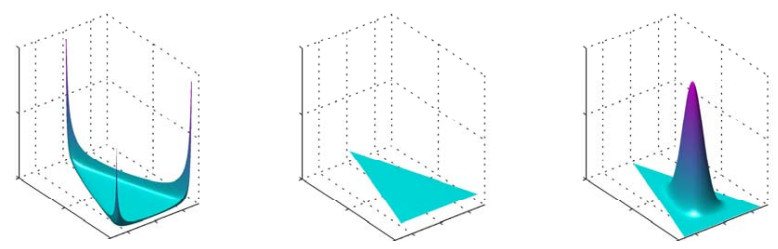
\includegraphics[width= 1.0\textwidth]{figures//dirichlet_chap5.jpg}\\
  	\caption{三维空间狄利克雷分布密度图}\label{fig:dirichlet_chap5}
	\end{figure}
	
\end{itemize}

在一般的主题模型如LDA中,初始假设每一个主题是基于所有词的一个均匀狄利克雷分布(参数为$\beta$)。而正如George Box讽刺说道:所有的模型都是错的(``all models are wrong''),特别是对于贝叶斯模型(Bayesian model)\cite{box1976science}。因此,这个先验假设往往与实际情况不符合,因为在实际中一个主题只高概率关系到少数词,而随机初始化也无法保证主题的多样性。尽管主题模型的最终目的是学习到主题和词的后验概率关系,但是先验概率对于整个主题模型的收敛速度以及收敛结果有着非常重要的影响。

\subsection{词向量聚类先验潜在狄利克雷分布}\label{subsec_priorLDA_chap5}

\begin{figure}[htbp]
  \centering
  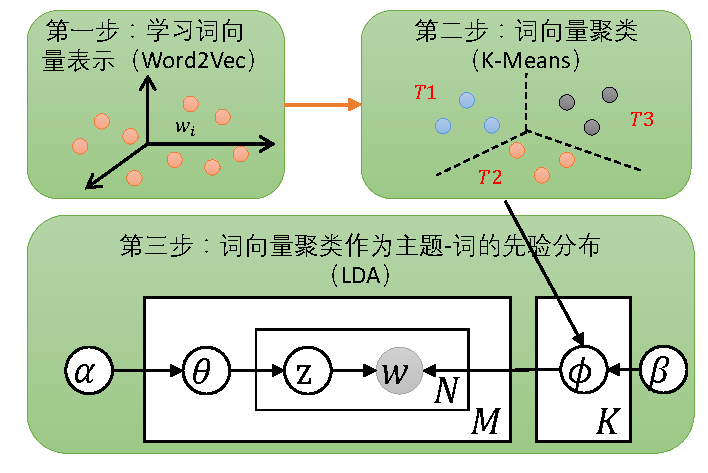
\includegraphics[width= 1.0\textwidth]{figures//word_cluster_prior_chap5.pdf}\\
  \caption{词向量聚类先验潜在狄利克雷分布}\label{fig:wc_prior_chap5}
\end{figure}

幸运的是在前面章节中,我们可以从大规模的未标注语料中通过非监督方法学习到词的分布式向量表示,而且词的向量表示可以表征词的语义信息。因此,我们可以利用先前学到的词向量表示提供给主题模型作为先验。最简单直接的想法就是如图\ref{fig:wc_prior_chap5}所示:

	\begin{enumerate}
	\item \textbf{学习词向量表示}:利用词向量表示方法如Word2Vec\footnote{https://code.google.com/archive/p/word2vec/}学习每个词的向量表示。
	\item \textbf{词向量聚类}:对词向量根据主题模型的主题数进行K-Means聚类。
	\item \textbf{词向量聚类作为先验}:依据词向量聚类结果,在主题模型如LDA初始化词的主题阶段,将词的主题设置为聚类的类别ID。之后依据原有LDA主题模型过程进行建模。
	\end{enumerate}
	
我们期望通过在LDA训练初始阶段采用词向量聚类的结果来代替原来的随机初始化过程,可以多方面优化LDA的主题建模结果:
	\begin{enumerate}
	\item \textbf{收敛速度}:一个好的初始化可以使得模型在参数求解过程中收敛速度加快;
	\item \textbf{收敛效果}:一个好的初始化可以使得模型能够找到更好的解,收敛结果更好;
	\item \textbf{主题一致性和多样性}:替代原有的狄利克雷先验,采用词向量K-Means聚类的结果作为主题-词的先验可以增加主题的一致性和多样性。
	\end{enumerate}

\section{词向量聚类先验实验与分析}\label{sec_exp_priorLDA_chap5}

在本部分,借助于$GibbsLDA++$\footnote{http://gibbslda.sourceforge.net/},我们实现了词向量聚类先验潜在狄利克雷分布(word embedding clustering prior LDA, wecpLDA)\footnote{https://github.com/NIULQfromNJU/nju-niulq-master-thesis/tree/master/code\%20datasets}。

\subsection{数据集与实验设置}\label{subsec_exp_priorLDA_datasets_chap5}

我们选用英语Gigaword\footnote{https://catalog.ldc.upenn.edu/LDC2011T07}作为训练数据来学习词向量表示以及运行主题模型。实际中,我们随机选择部分文档构造了对应的数据集,如下说明:

\begin{itemize}
\item \textbf{ltw\_100k}:从包含了$411032$文档数的Gigaword子目录ltw\_eng(Los Angeles Times)中选取了$100000$的文档,且每篇文档长度至少包含$1000$个字符。\textbf{ltw\_100k}数据集主要用来学习基本的词向量表示和构造后续数据集来运行主题模型。
\item \textbf{ltw\_10k}:从上述\textbf{ltw\_100k}数据集中随机抽取$10000$个文档来运行主题模型。
\item \textbf{ltw\_20k}:从上述\textbf{ltw\_100k}数据集中随机抽取$20000$个文档作为外部数据(external data)来进行主题一致性(Topic Coherence)评估。
\end{itemize}

\subsection{主题词评估}\label{subsec_exp_priorLDA_twords_chap5}

在任意主题模型对文档建模完成之后,我们会得到每一个主题关于所有词的概率分布$\Phi$。而对于所学习得到的每一个主题的好坏进行评估,最原始的任务是依据给定主题下的条件概率值排序,我们可以得到与每一个主题最相关的top $N$个主题词(Topic Words)。

\begin{figure}[htbp]
  \centering
  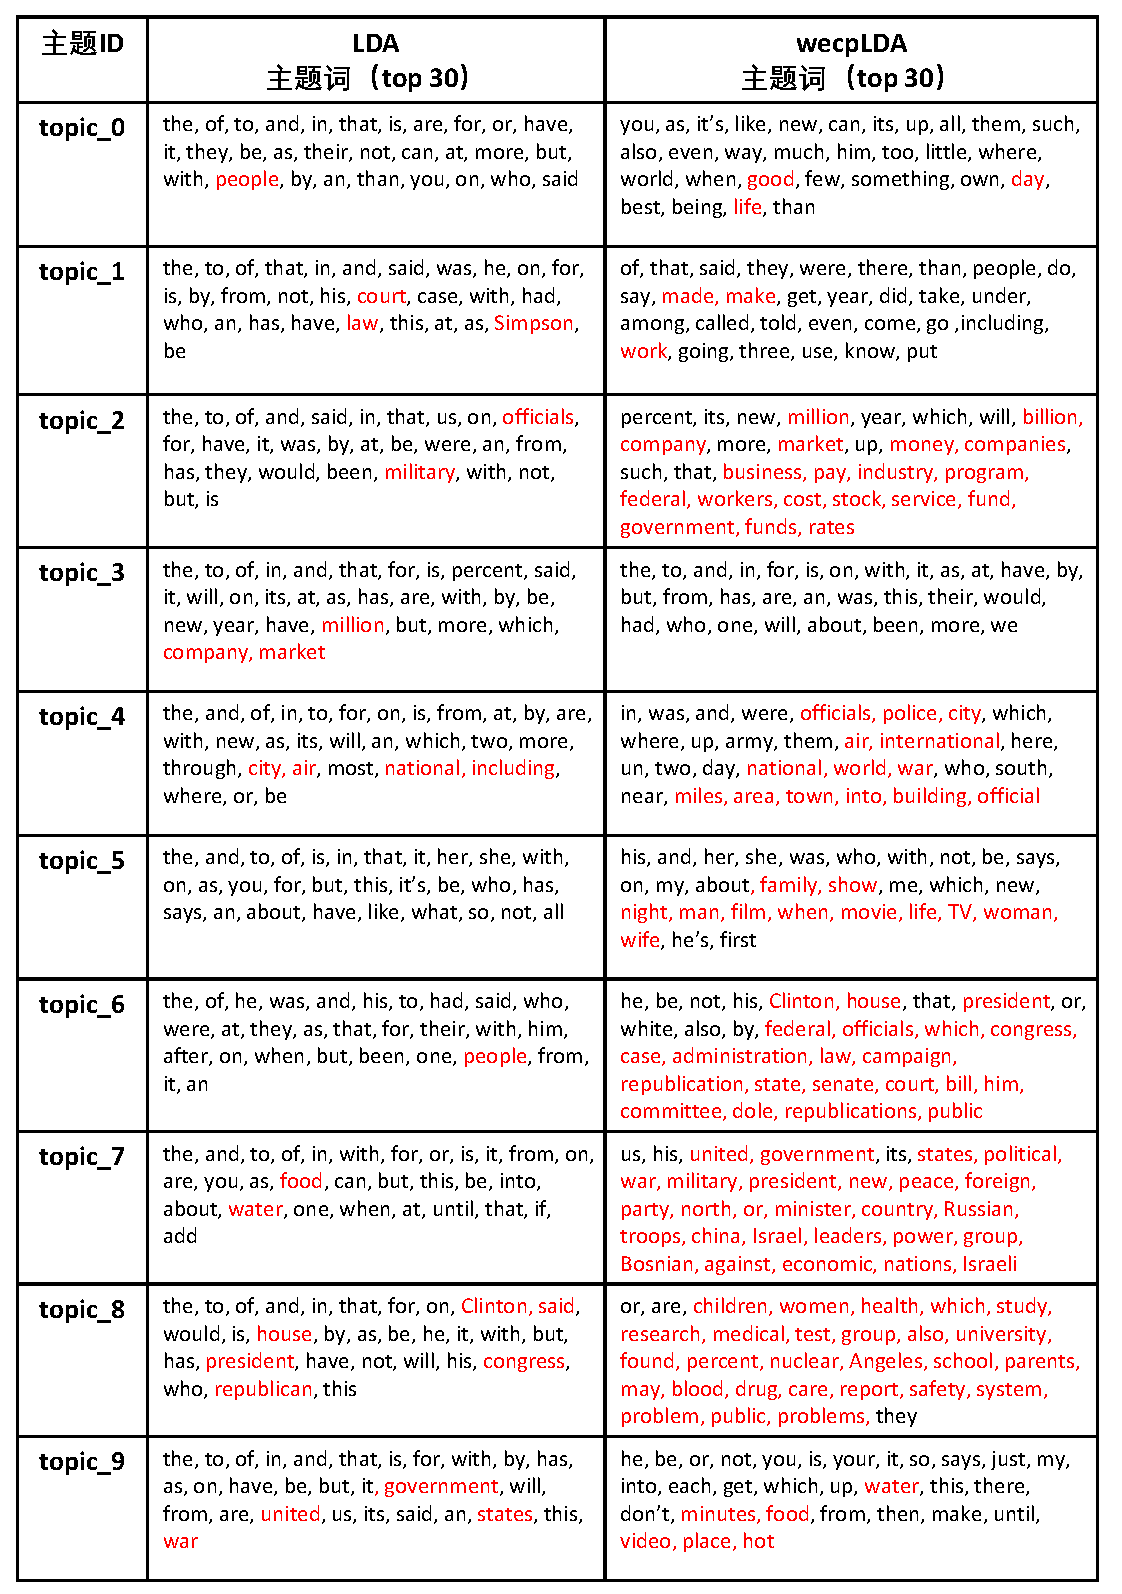
\includegraphics[width= 1.0\textwidth]{figures//twords_iter100_chap5.pdf}\\
  \caption{迭代次数为100时列举wecpLDA和LDA的主题词}\label{fig:twords_iter100_chap5}
\end{figure}

\begin{figure}[htbp]
  \centering
  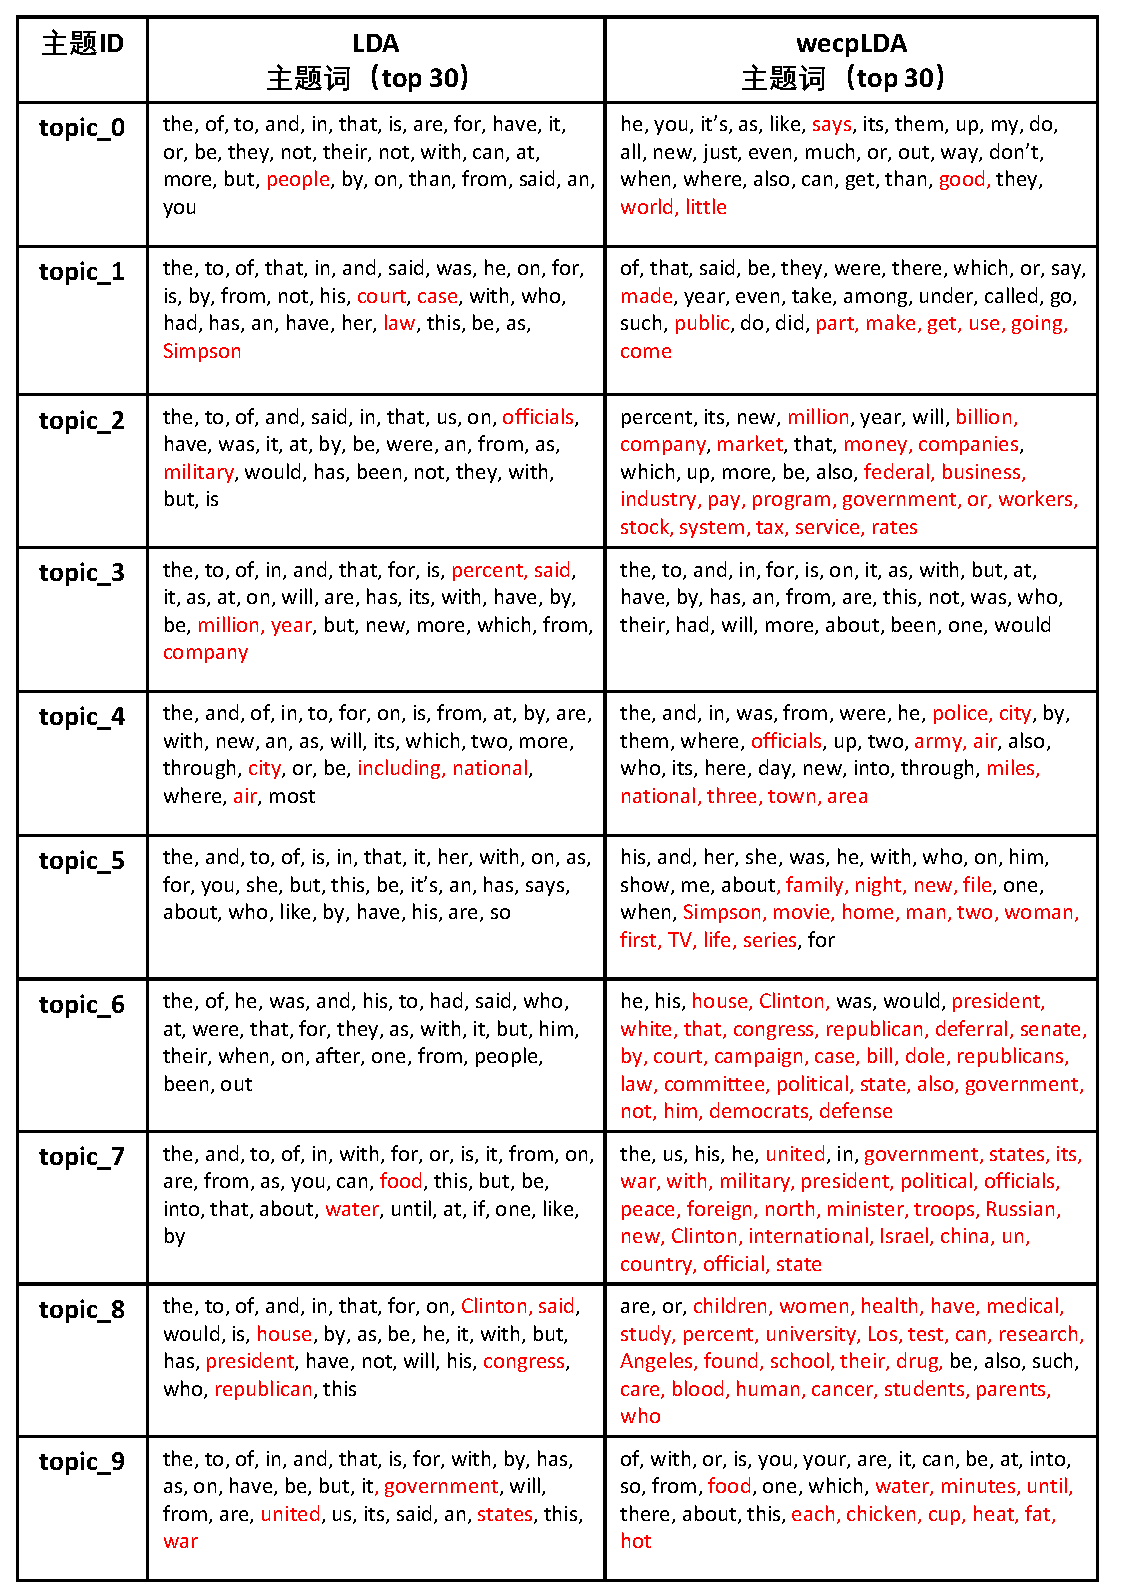
\includegraphics[width= 1.0\textwidth]{figures//twords_iter200_chap5.pdf}\\
  \caption{迭代次数为200时列举wecpLDA和LDA的主题词}\label{fig:twords_iter200_chap5}
\end{figure}

\begin{figure}[htbp]
  \centering
  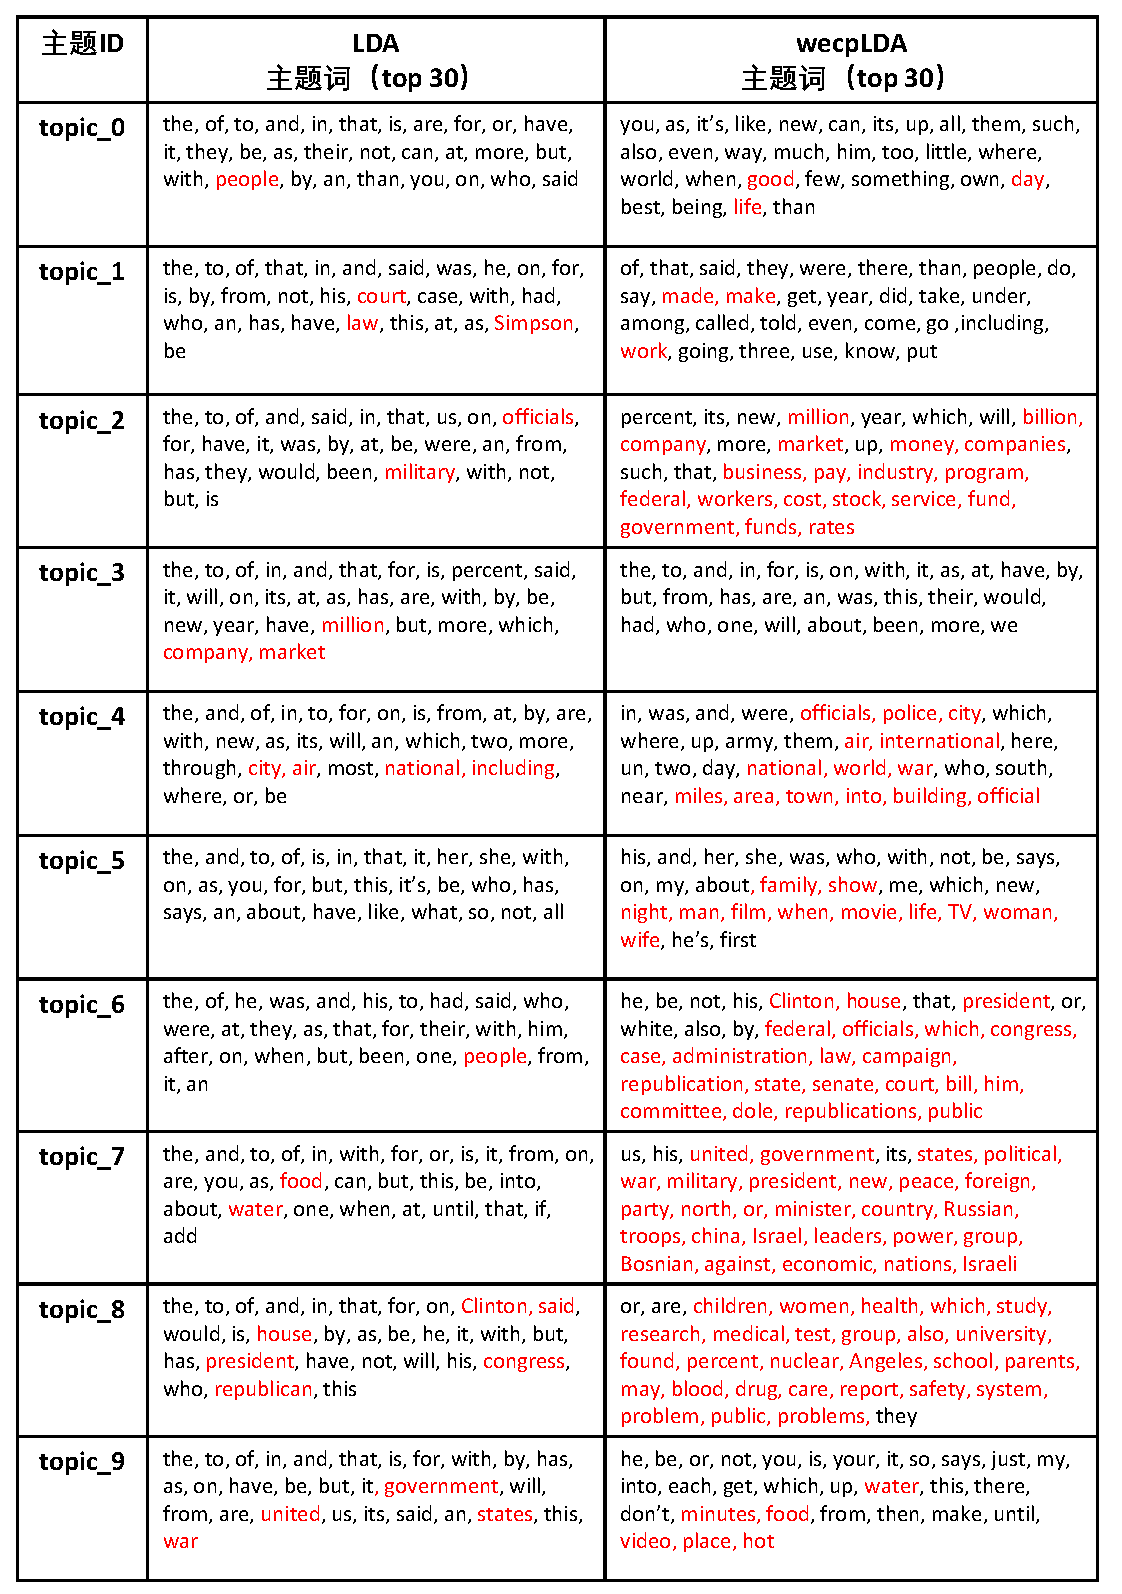
\includegraphics[width= 1.0\textwidth]{figures//twords_iter100_chap5.pdf}\\
  \caption{迭代次数为300时列举wecpLDA和LDA的主题词}\label{fig:twords_iter300_chap5}
\end{figure}


\subsection{主题一致性评估}\label{subsec_exp_priorLDA_tcoherence_chap5}

从一个统计主题模型学到的主题形式上是所有词的一个多项式分布,平常通过打印出主题中最相关的$N$个词。这些top-$N$通常提供了足够的信息来决定主旨领域和主题的解释,并且可以区别不同的主题。然而,从稀疏(sparse)或者带噪音(noise)的数据学习到的主题通常一致性较差,较难解释,并且通常是无用的。因此在本节,我们通过分布式词向量的聚类结果来作为主题模型中主题-词的先验分布,期望改善之后主题模型的结果中对于同一个主题的top-$N$个主题词是一致的。

因此,在实验中我们可以评估主题一致性(Topic Coherence)。主题一致性-意味着语义一致性-是基于词的语义信息人工做出的质量判断,而且不能够通过那些将词作为可调换的符号的基于模型的统计度量。幸运的是,最近的工作显示出利用基于逐点互信息(pointwise mutual information, PMI)得分可以自动评估接近人的准确率的主题一致性\cite{newman2010automatic,newman2010evaluating}。PMI-Score受到度量所有top-$N$主题词词对之间的词关联性激发,PMI-Score按如下方式定义:
	\begin{equation}
	PMI-Score(\textbf{w})=\frac{1}{N(N-1)/2}\sum_{i<j}PMI(w_i, w_j),ij\in \{1, ..., N\}
	\end{equation}
	其中
	\begin{equation}
	PMI(w_i, w_j)=log\frac{P(w_i, w_j)}{P(w_i)P(w_j)}
	\end{equation}
这里$N(N-1)/2$是top-$N$个主题词之间不同的词对数量,$P(w_i, w_j)$,$P(w_i)$和$P(w_j)$分别是语料中词$w_i$和$w_j$共同出现在一个上下文窗口(通常窗口大小设置为$k=10$\cite{newman2010automatic})的概率,词$w_i$出现的概率和词$w_j$出现的概率。一个关键点是这个得分采用外部数据(external data)-这个数据没有在主题建模过程中使用。这个数据可以有多种多样的来源,比如我们随机抽取的不同于主题建模数据集\textbf{ltw\_10k}的数据集\textbf{ltw\_20k}。

\subsection{实验与分析}\label{subsec_exp_results_chap5}

在实验中,我们首先在数据集\textbf{ltw\_100k}上运行Word2Vec学习词的向量表示。紧接着我们在数据集\textbf{ltw\_10k}上运行LDA,并且设置主题数$K=10$,迭代次数$iter=300$,并且每隔$100$次迭代就保存模型。在wecpLDA运行之前,我们先对之前学习到的词向量进行K-Means聚类,设置类别$K=10$,保持与主题模型主题数一致。之后采用K-Means的聚类结果作为先验来对词的主题进行初始化。随后过程跟LDA相同,均采用吉布斯采样,参数设置也保持一致。

\begin{table}[htbp]
\centering
\caption{LDA和wecpLDA主题模型评估结果对比}
\label{tab:exp_results_chap5}
\begin{tabular}{|c|c|c|}
\hline
\textbf{主题模型评估} & \textbf{LDA} & \textbf{wecpLDA} \\ \hline
初始化方法			 & 狄利克雷先验随机初始化	& 词向量K-Means聚类先验初始化	\\ \hline
收敛速度            & 慢            & 快                \\ \hline
收敛结果            & 差            & 好                \\ \hline
主题一致性           & 差            & 好                \\ \hline
主题多样性           & 差            & 好                \\ \hline
处理稀疏和噪音数据	& 差	 & 好		  \\ \hline
\end{tabular}
\end{table}

关于实验结果,如图\ref{fig:twords_iter100_chap5},\ref{fig:twords_iter200_chap5}和\ref{fig:twords_iter300_chap5}所示,分别是LDA和wecpLDA迭代次数为$100$,$200$和$300$时依据条件概率值列举$K=10$个主题所包含的top-$N=30$主题词(其中红色高亮突出具有实际意义的词)。由主题词的结果可以看出,LDA在面对这类未去除停用词(stop words)的噪音数据集时,这些停用词通常是作为高频词,而LDA的结果会偏向于这些高频词,因此每个主题所包含的主题词结果较差。而wecpLDA采用了词向量聚类先验初始化的结果明显要好很多,比LDA的主题词结果更有意义。单从这些主题词的结果来看,仅仅改变初始化过程就可以明显改善LDA的运行结果。因此我们通过人工判断对LDA和wecpLDA进行了多方面的评估,结果如表\ref{tab:exp_results_chap5}所示。

\section{词向量加强的潜在狄利克雷分布}\label{sec_enhanced_lda_chap5}

在前面章节中,仅仅利用词向量聚类先验来初始化就使得wecpLDA的收敛速度、收敛结果以及主题的多样性和一致性等大为改善。但是wecpLDA对于词向量的利用仅仅限于主题模型的初始化阶段,后续过程依旧采用原有LDA的吉布斯采样来推断。
 
在本节内容,我们将深入探索如何将词向量表示应用到主题模型中。首先,我们修改原有LDA的图模型结构,引入上下文隐藏变量$c$,提出上下文感知的潜在狄利克雷分布(Context-aware LDA)。之后在上下文感知LDA的基础上引入词向量表示来进一步优化整个主题模型,并提出词向量加强的潜在狄利克雷分布(word embedding enhanced LDA)模型。
 
\subsection{上下文感知的潜在狄利克雷分布}\label{subsec_context_aware_lda_chap5}

\begin{figure}[htbp]
\centering
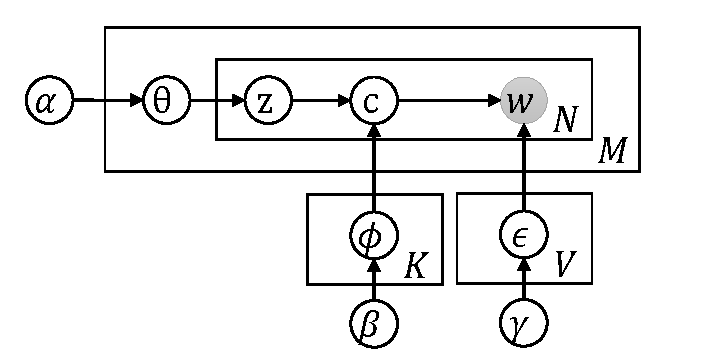
\includegraphics[width= 1.0\textwidth]{figures//caLDA_chap5.pdf}\\
\caption{上下文感知LDA的图模型表示}\label{fig:caLDA_chap5}
\end{figure}

如图\ref{fig:caLDA_chap5}所示,上下文感知潜在狄利克雷分布(Context-aware LDA, caLDA)是一个生成式概率模型。其基本的思想是文档表示为隐藏主题的混合分布$\theta$,每一个主题表示为所有上下文词的概率分布$\phi$,而每一个上下文词同时表示为词汇表中所有词的概率分布$\epsilon$。caLDA的生成过程如下:
	\begin{enumerate}
	\item 对每一个文档$For\ d=1, ..., M: \theta_{d}\sim Dir(\alpha)$
	\item 对每一个主题$For\ k=1, ..., K: \phi_{k}\sim Dir(\beta)$
	\item 对每一个上下文词$For\ v=1, ..., V: \epsilon_{v}\sim Dir(\gamma)$
	\item 对文档中出现的每一个词$For\ n=1, ..., N:$
		\begin{itemize}
		\item 当前主题$z_{n}\sim Mult(\theta_{d})$
		\item 当前上下文词$c_{n}\sim Mult(\phi_{z_{n}})$
		\item 当前词$w_{n}\sim Mult(\epsilon_{c_{n}})$
		\end{itemize}
	\end{enumerate}
这里$\alpha$,$\beta$和$\gamma$是超参,分别对应概率分布$\theta$,$\phi$和$\epsilon$的狄利克雷先验,$Dir()$表示狄利克雷分布,$Mult()$为多项式分布。

我们都知道在LDA中,直接对整个模型进行准确推断(exact inference)是棘手的\cite{blei2003latent}。因此通常的处理办法是借助于近似推断技术,包括变分推断(variational inference)和马尔可夫链蒙特卡洛(Markov chain Monte Carlo, MCMC)方法等。其中变分推断引入变分空间将整个问题转化为一个优化问题,而MCMC则通过采样等随机游走方法来寻求收敛的最优解。MCMC中最简单的方法则是吉布斯采样(Gibbs sampling),因此在这里我们选择吉布斯采样来推断主题模型的参数\cite{griffiths2004finding}。caLDA的吉布斯采样过程如下:
	\begin{enumerate}
	\item 	对文档中的每一个观测词$w_i$,采样其上下文词$c_i$:
			\begin{equation}\label{eq:caLDA_gb_c_chap5}
			P(c_i=v|\mathbf{c_{-i}, w, z})\propto \frac{n_{-i, v}^{(w_i)}+\gamma}{n_{-i, v}^{(.)}+V\gamma}\cdot \frac{n_{-i, v}^{(z_i)}+\beta}{n_{-i, .}^{(z_i)}+V\beta}
			\end{equation}
	这里$n_{-i}^{(.)}$是一个不包括当前$c_i$赋值的计数。上述结果也是十分的直观,第一个比例表示当前词$w_i$在预测上下文词$v$下的概率值,第二个比例表示预测上下文词$v$在当前主题$z_i$下的概率值。
	\item 	根据前一步采样得到的上下文词$c_i$,采样其主题$z_i$:
			\begin{equation}\label{eq:caLDA_gb_z_chap5}
			P(z_i=k|\mathbf{z_{-i}, w, c})\propto \frac{n_{-i, k}^{(c_i)}+\beta}{n_{-i, k}^{(.)}+V\beta}\cdot \frac{n_{-i, k}^{(d_i)}+\alpha}{n_{-i, .}^{(d_i)}+K\alpha}
			\end{equation}
	这里$n_{-i}^{(.)}$是一个不包括当前$z_i$赋值的计数。上述结果也是十分的直观,第一个比例表示当前上下文词$c_i$在预测主题$k$下的概率值,第二个比例表示预测主题$k$在当前文档$d_i$下的概率值。
	\end{enumerate}

有了从后验分布$P(\textbf{c}|\textbf{w, z})$和$P(\textbf{z}|\textbf{w, c})$吉布斯采样得到的样本集,每一个单独的上下文词和主题中相互独立的统计量可以通过整合所有样本集来计算。对于任意一个样本,我们可以估计从$\textbf{c}$和$\textbf{z}$的值来统计$\theta$,$\phi$和$\epsilon$:
	\begin{enumerate}
	\item 词$w$在上下文词$c$下的概率值为:
		\begin{equation}
		\hat{\epsilon}_{c}^{(w)}=\frac{n_c^{(w)}+\gamma}{n_c^{(.)}+V\gamma}
		\end{equation}
	\item 上下文词$c$在主题$j$下的概率值为:
		\begin{equation}
		\hat{\phi}_{j}^{(c)}=\frac{n_j^{(c)}+\beta}{n_j^{(.)}+V\beta}
		\end{equation}
	\item 主题$j$在文档$d$中的概率值为:
		\begin{equation}
		\hat{\theta}_{j}^{(d)}=\frac{n_{j}^{(d)}+\alpha}{n_{.}^{(d)}+K\alpha}
		\end{equation}	
	\end{enumerate}
	这些值基于$\textbf{w}$,$\textbf{c}$和$\textbf{z}$可以用来估计新出现的$w$,$c$和$z$。

\subsection{词向量加强的潜在狄利克雷分布}\label{subsec_enhanced_lda_chap5}
 
\begin{figure}[htbp]
\centering
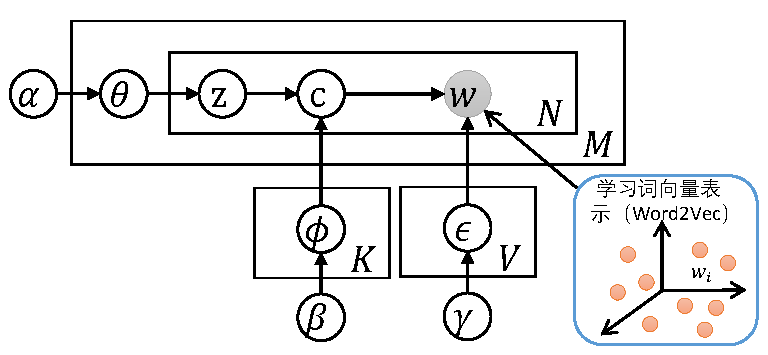
\includegraphics[width= 1.0\textwidth]{figures//weeLDA_chap5.pdf}\\
\caption{词向量加强LDA的图模型表示}\label{fig:weeLDA_chap5}
\end{figure}

如图\ref{fig:weeLDA_chap5}所示,词向量加强潜在狄利克雷分布(word embedding enhanced LDA, weeLDA)在上下文词$c$生成当前观测词$w$时可以利用学习到的词向量表示来替代原来的狄利克雷先验分布。这里简单假设词向量生成上下文词-词的概率分布为$Dis()$,weeLDA的生成过程如下:
	\begin{enumerate}
	\item 对每一个文档$For\ d=1, ..., M: \theta_{d}\sim Dir(\alpha)$
	\item 对每一个主题$For\ k=1, ..., K: \phi_{k}\sim Dir(\beta)$
	\item 对每一个上下文词$For\ v=1, ..., V: \epsilon_{v}\sim Dir(\gamma)$
	\item 对每一个上下文词$For\ v=1, ..., V: \epsilon'_{v}\sim Dis()$
	\item 对文档中出现的每一个词$For\ n=1, ..., N:$
		\begin{itemize}
		\item 当前主题$z_{n}\sim Mult(\theta_{d})$
		\item 当前上下文词$c_{n}\sim Mult(\phi_{z_{n}})$
		\item 当前词$w_{n}\sim Mult(\epsilon_{c_{n}}) \cdot Dis((\epsilon'_{c_{n}})$
		\end{itemize}
	\end{enumerate}
	
类似地,weeLDA的吉布斯采样过程如下:
	\begin{enumerate}
	\item 	对文档中的每一个观测词$w_i$,采样其上下文词$c_i$:
			\begin{equation}\label{eq:caLDA_gb_c_chap5}
			P(c_i=v|\mathbf{c_{-i}, w, z})\propto \frac{n_{-i, v}^{(w_i)}+\gamma}{n_{-i, v}^{(.)}+V\gamma}\cdot \frac{\exp(\mathbf{v} \cdot \mathbf{w_{i}})}{\sum_{c\in C}\exp(\mathbf{c} \cdot \mathbf{w_{i}})} \cdot \frac{n_{-i, v}^{(z_i)}+\beta}{n_{-i, .}^{(z_i)}+V\beta}
			\end{equation}
			这里对于分布$Dis()$采用了Softmax函数,$\mathbf{v}$,$\mathbf{c}$和$\mathbf{w_i}$分别表示上下文词$v$,任意上下文词$c$和当前观测词$w_i$的词向量表示。这里$n_{-i}^{(.)}$是一个不包括当前$c_i$赋值的计数。上述结果也是十分的直观,第一个和第二个比例表示当前词$w_i$在预测上下文词$v$下的概率值,第三个比例表示预测上下文词$v$在当前主题$z_i$下的概率值。
	\item 	根据前一步采样得到的上下文词$c_i$,采样其主题$z_i$:
			\begin{equation}\label{eq:caLDA_gb_z_chap5}
			P(z_i=k|\mathbf{z_{-i}, w, c})\propto \frac{n_{-i, k}^{(c_i)}+\beta}{n_{-i, k}^{(.)}+V\beta}\cdot \frac{n_{-i, k}^{(d_i)}+\alpha}{n_{-i, .}^{(d_i)}+K\alpha}
			\end{equation}
			这里$n_{-i}^{(.)}$是一个不包括当前$z_i$赋值的计数。上述结果也是十分的直观,第一个比例表示当前上下文词$c_i$在预测主题$k$下的概率值,第二个比例表示预测主题$k$在当前文档$d_i$下的概率值。
	\end{enumerate}
	
有了从后验分布$P(\textbf{c}|\textbf{w, z})$和$P(\textbf{z}|\textbf{w, c})$吉布斯采样得到的样本集,类似地,我们可以估计从$\textbf{c}$和$\textbf{z}$的值来统计$\theta$,$\phi$和$\epsilon$:
	\begin{enumerate}
	\item 词$w$在上下文词$c$下的概率值为:
		\begin{equation}
		\hat{\epsilon}_{c}^{(w)}=\frac{n_c^{(w)}+\gamma}{n_c^{(.)}+V\gamma}
		\end{equation}
	\item 上下文词$c$在主题$j$下的概率值为:
		\begin{equation}
		\hat{\phi}_{j}^{(c)}=\frac{n_j^{(c)}+\beta}{n_j^{(.)}+V\beta}
		\end{equation}
	\item 主题$j$在文档$d$中的概率值为:
		\begin{equation}
		\hat{\theta}_{j}^{(d)}=\frac{n_{j}^{(d)}+\alpha}{n_{.}^{(d)}+K\alpha}
		\end{equation}	
	\end{enumerate}
	同样地,这些值基于$\textbf{w}$,$\textbf{c}$和$\textbf{z}$可以用来估计新出现的$w$,$c$和$z$。
	
本节重点在于基于利用外部的词向量表示来改善主题模型效果的思想,修改了LDA的图模型表示,并提出了对应的上下文感知的LDA(caLDA)和词向量加强的LDA(weeLDA),并且给出了各自模型的吉布斯采样方法。


\section{本章小结}\label{sec_conclusions_chap5}

本章内容的出发点是基于词向量表示和主题模型各自的优势特点,分析主题模型存在的问题,并且希望通过学习到的词向量表示来提升主题模型的效果。特别地,本章的贡献如下:

\begin{itemize}
\item 分析了LDA中初始化阶段采用狄利克雷先验分布的不足,提出利用词向量K-Means聚类的结果来替代狄利克雷分布的模型。通过实验分析,对词向量聚类先验LDA和原有LDA在收敛速度、收敛效果、主题一致性和多样性等方面作了对比分析。
\item 深入探索了词向量表示与主题模型的融合应用,通过修改原有LDA的图模型表示,分别提出了上下文感知的潜在狄利克雷分布(caLDA)和词向量加强的潜在狄利克雷分布(weeLDA)。并且借鉴LDA中吉布斯采样推断技术,分别给出各自模型的吉布斯采样方法。
\end{itemize}

在未来工作中,我们期望分别实现caLDA和weeLDA,并且在收敛效果、主题一致性和多样性等多个方面对其进行定性和定量的分析。

%%%%%%%%%%%%%%%%%%
%%%%%%%%%%%%%%%%%%%%%%%%%%%%%%%%%%%%%%%%%%%%%%%%%%%%%%%%%%%%%%%%%%%%%%%%%%%%%%%
% 学位论文的正文应以《结论》作为最后一章
\chapter{总结与展望}\label{chapter6_concludes}

基于深度学习技术在人工智能领域取得的重大突破,本文集中对于深度神经网络在自然语言处理领域中文本表示与主题模型等问题进行了研究。具体地,
\begin{itemize}
\item 在第\ref{chapter2_nnlm_word_representations}章语言模型与词向量表示中,主要介绍本文的背景工作,包括传统N-Gram统计语言模型、Bengio等人在2003年提出的神经网络语言模型\cite{bengio2003neural}以及Mikolov等人在2013年提出的基于神经网络语言模型学习分布式词向量表示的模型Word2Vec\cite{mikolov2013efficient,mikolov2013distributed,mikolov2013linguistic}。
\item 在第\ref{chapter3_topic_representations}章学习主题的向量表示中,主要工作是借助于潜在狄利克雷分布(Latent Dirichlet Allocation, LDA)挖掘到词的主题(Topic)信息,将Word2Vec扩展至学习分布式主题向量表示,并且提出了模型Topic2Vec。并且通过主题词实验对比了Topic2Vec和LDA,结果表明Topic2Vec的结果可以更好的表征主题。
\item 在第\ref{chapter4_word_attributes}章联合学习词和属性的向量表示中,主要工作是将Word2Vec扩展到一个能够联合学习词(Word)和属性(Attributes)分布式向量表示的统一框架,其中重点引入了三类词属性:词元(Lemma)、主题(Topic)、文档(Document),基于该框架实现:(1)学习主题Topic的分布式表示、(2)学习文档Document的分布式表示和(3)利用词元和主题信息来提升词向量表示。针对上述各类向量表示分别进行了实验对比分析,结果表明该框架不仅可以学习到属性的分布式表示,而且可以利用属性知识来提高原来词向量表示。另外,该框架易于扩展,可以学习更多其他的词属性的分布式表示。
\item 在第\ref{chapter5_embedding_topic_model}章词向量加强的主题模型中,主要工作是基于词向量表示可以表示词的句法和语义信息以及主题模型存在的问题,将词向量表示应用到主题模型中来提升主题模型。首先采用词向量聚类结果作为LDA主题-词的先验分布,提出了词向量聚类先验潜在狄利克雷分布(wecpLDA)。之后修改LDA的图模型结构,提出了对应的上下文感知潜在狄利克雷分布(caLDA)以及词向量加强的潜在狄利克雷分布(weeLDA)。
\end{itemize}

文本表示和主题建模作为基础任务在自然语言处理中扮演着重要的角色,在未来工作中,我们将继续深入研究深度学习技术即深度神经网络在自然语言处理特别是文本向量表示和主题建模等问题上的应用。

%%%%%%%%%%%%%%%%%%%%%%%%%%%%%%%%%%%%%%%%%%%%%%%%%%%%%%%%%%%%%%%%%%%%%%%%%%%%%%%
% 致谢,应放在《结论》之后
\begin{acknowledgement}

%回想来到自然语言处理研究组之初,自己对于自然语言处理、机器学习、人工智能等概念知之甚少,但是内心却是充满兴趣和期待。而且,对于这些理论模型方面甚至整个人工智能领域的发展的关注度丝毫不减。面对整个人工智能领域广泛的科学知识,三年时间显得很短,自己所学到的知识还远远不够,在以后的工作生活中仍需坚持不断学习的态度,争取有所作为。

岁月如梭,光阴荏苒,不经意间三年的研究生生涯即将结束。在这三年的学习生活中,从基础的自然语言处理任务到广泛的机器学习理论模型、统计方法等,自己都收获颇丰,学到了很多的知识,找到很多自己感兴趣的方向。 对于这三年的研究生生活,自己也感到特别幸运。幸运的是可以安心学习知识,找到自己喜欢的研究方向,完成自己的学业;幸运的是可以跟实验室的老师和同学们愉快的相处;幸运的是可以跟小伙伴们建立更加深厚的友谊。因此,在这里我想对所有帮助支持我的人表示感谢。

首先,我想感谢我的导师戴新宇副教授。感谢戴老师接受我来到自然语言处理研究组学习,并且在之后的三年中,对于我的学习生活、研究工作等多方面给予了极大的指导和帮助。还有,我想感谢南京大学自然语言处理研究组的陈家骏教授、黄书剑老师和尹存燕老师,感谢老师们对于我三年学习生活所给予的指导和鼓励。

其次,我想感谢实验室的师兄邹远航、陈华栋、周浩和师姐潘林林。特别地,感谢邹远航师兄在我来研究组之初对于我的学习内容给予的指导,并且在找实习和工作期间给予的帮助和鼓励。还有,我想特别感谢同届的胡光能、程川、程善伯、黄家君和周逸初,祝福他们以后的学习和工作越来越好。还要感谢下一届可爱的师弟师妹,他们是尚迪、李小婉、郁振庭、汤莲瑞、季红洁、周启元和王韶杰,祝福他们的学习更加进步。

另外,我想感谢学习之余一起玩耍的小伙伴们,他们是缪峥、蒋继东、刘锐奇、刘超、向文君、蒋哲翎、姜成樾、葛奕和丁丽,感谢他们带来的欢乐,祝福他们以后的工作和学习生活更加美好。还有我想感谢腾讯CDG检索策略组的applelin和frankiehu等,感谢他们在实习期间给予我的鼓励和帮助。

最后,我想特别感谢我的家人。感谢我的父母在这二十多年的成长和学习历程中给予的关怀和无私的爱。感谢我的弟弟,感谢他的懂事和一直以来对我的鼓励和支持。

只言片语道不尽我的感激之情,谨以此文献给所有支持我的关心、支持、帮助过我的人。


\end{acknowledgement}

%%%%%%%%%%%%%%%%%%%%%%%%%%%%%%%%%%%%%%%%%%%%%%%%%%%%%%%%%%%%%%%%%%%%%%%%%%%%%%%


% 参考文献。应放在\backmatter之前。
% 推荐使用BibTeX,若不使用BibTeX时注释掉下面一句。
\nocite{*}
\bibliography{niu-thesis}
% 不使用 BibTeX
%\begin{thebibliography}{2}
%
%\bibitem{deng:01a}
%{邓建松,彭冉冉,陈长松}.
%\newblock {\em \LaTeXe{}科技排版指南}.
%\newblock 科学出版社,书号:7-03-009239-2/TP.1516, 北京, 2001.
%
%\bibitem{wang:00a}
%王磊.
%\newblock {\em \LaTeXe{}插图指南}.
%\newblock 2000.
%\end{thebibliography}

% 附录,必须放在参考文献后,backmatter前
%\appendix
%\chapter{图论基础知识}

%%%%%%%%%%%%%%%%%%%%%%%%%%%%%%%%%%%%%%%%%%%%%%%%%%%%%%%%%%%%%%%%%%%%%%%%%%%%%%%
% 书籍附件
\backmatter
%%%%%%%%%%%%%%%%%%%%%%%%%%%%%%%%%%%%%%%%%%%%%%%%%%%%%%%%%%%%%%%%%%%%%%%%%%%%%%%
% 作者简历与科研成果页,应放在backmatter之后
\begin{resume}
% 论文作者身份简介,一句话即可。
\begin{authorinfo}
\noindent 牛力强,男,汉族,1991年10月出生,出生于甘肃省甘谷县。
\end{authorinfo}
% 论文作者教育经历列表,按日期从近到远排列,不包括将要申请的学位。
\begin{education}
\item[2013年9月 --- 2016年6月] 南京大学计算机科学与技术系 \hfill 硕士
\item[2009年9月 --- 2013年6月] 南京大学计算机科学与技术系 \hfill 本科
\end{education}
% 论文作者在攻读学位期间所发表的文章的列表,按发表日期从近到远排列。
\begin{publications}
\item Liqiang Niu, Xin-Yu Dai, Shujian Huang, and Jiajun Chen. A Unified Framework for Jointly Learning Distributed Representations of Word and Attributes. In Proceedings of 7th Asian Conference on Machine Learning (ACML 2015) November 20-22, 2015, Hong Kong, JMLR: Workshop and Conference Proceedings 45:143–156, 2015
\item Liqiang Niu, Xinyu Dai, Jianbing Zhang, and Jiajun Chen. Topic2Vec: Learning Distributed Representations of Topics. In Proceedings of 2015 International Conference on Asian Language Processing (IALP 2015) pp. 193-196, 24-25 October, 2015, Suzhou, China
\end{publications}
% 论文作者在攻读学位期间参与的科研课题的列表,按照日期从近到远排列。
\begin{projects}
\item 国家自然科学基金面上项目``无线传感器网络在知识获取过程中的若干安全问题研究''
(课题年限~2010年1月 --- 2012年12月),负责位置相关安全问题的研究。
\item 江苏省知识创新工程重要方向项目下属课题``下一代移动通信安全机制研究''
(课题年限~2010年1月 --- 2010年12月),负责LTE/SAE认证相关的安全问题研究。
\end{projects}
\end{resume}

%%%%%%%%%%%%%%%%%%%%%%%%%%%%%%%%%%%%%%%%%%%%%%%%%%%%%%%%%%%%%%%%%%%%%%%%%%%%%%%
% 生成《学位论文出版授权书》页面,应放在最后一页
\makelicense


%%%%%%%%%%%%%%%%%%%%%%%%%%%%%%%%%%%%%%%%%%%%%%%%%%%%%%%%%%%%%%%%%%%%%%%%%%%%%%%
\end{document}
